% Figures
\afterpage{
    \begin{figure}[t!]
        \centering
        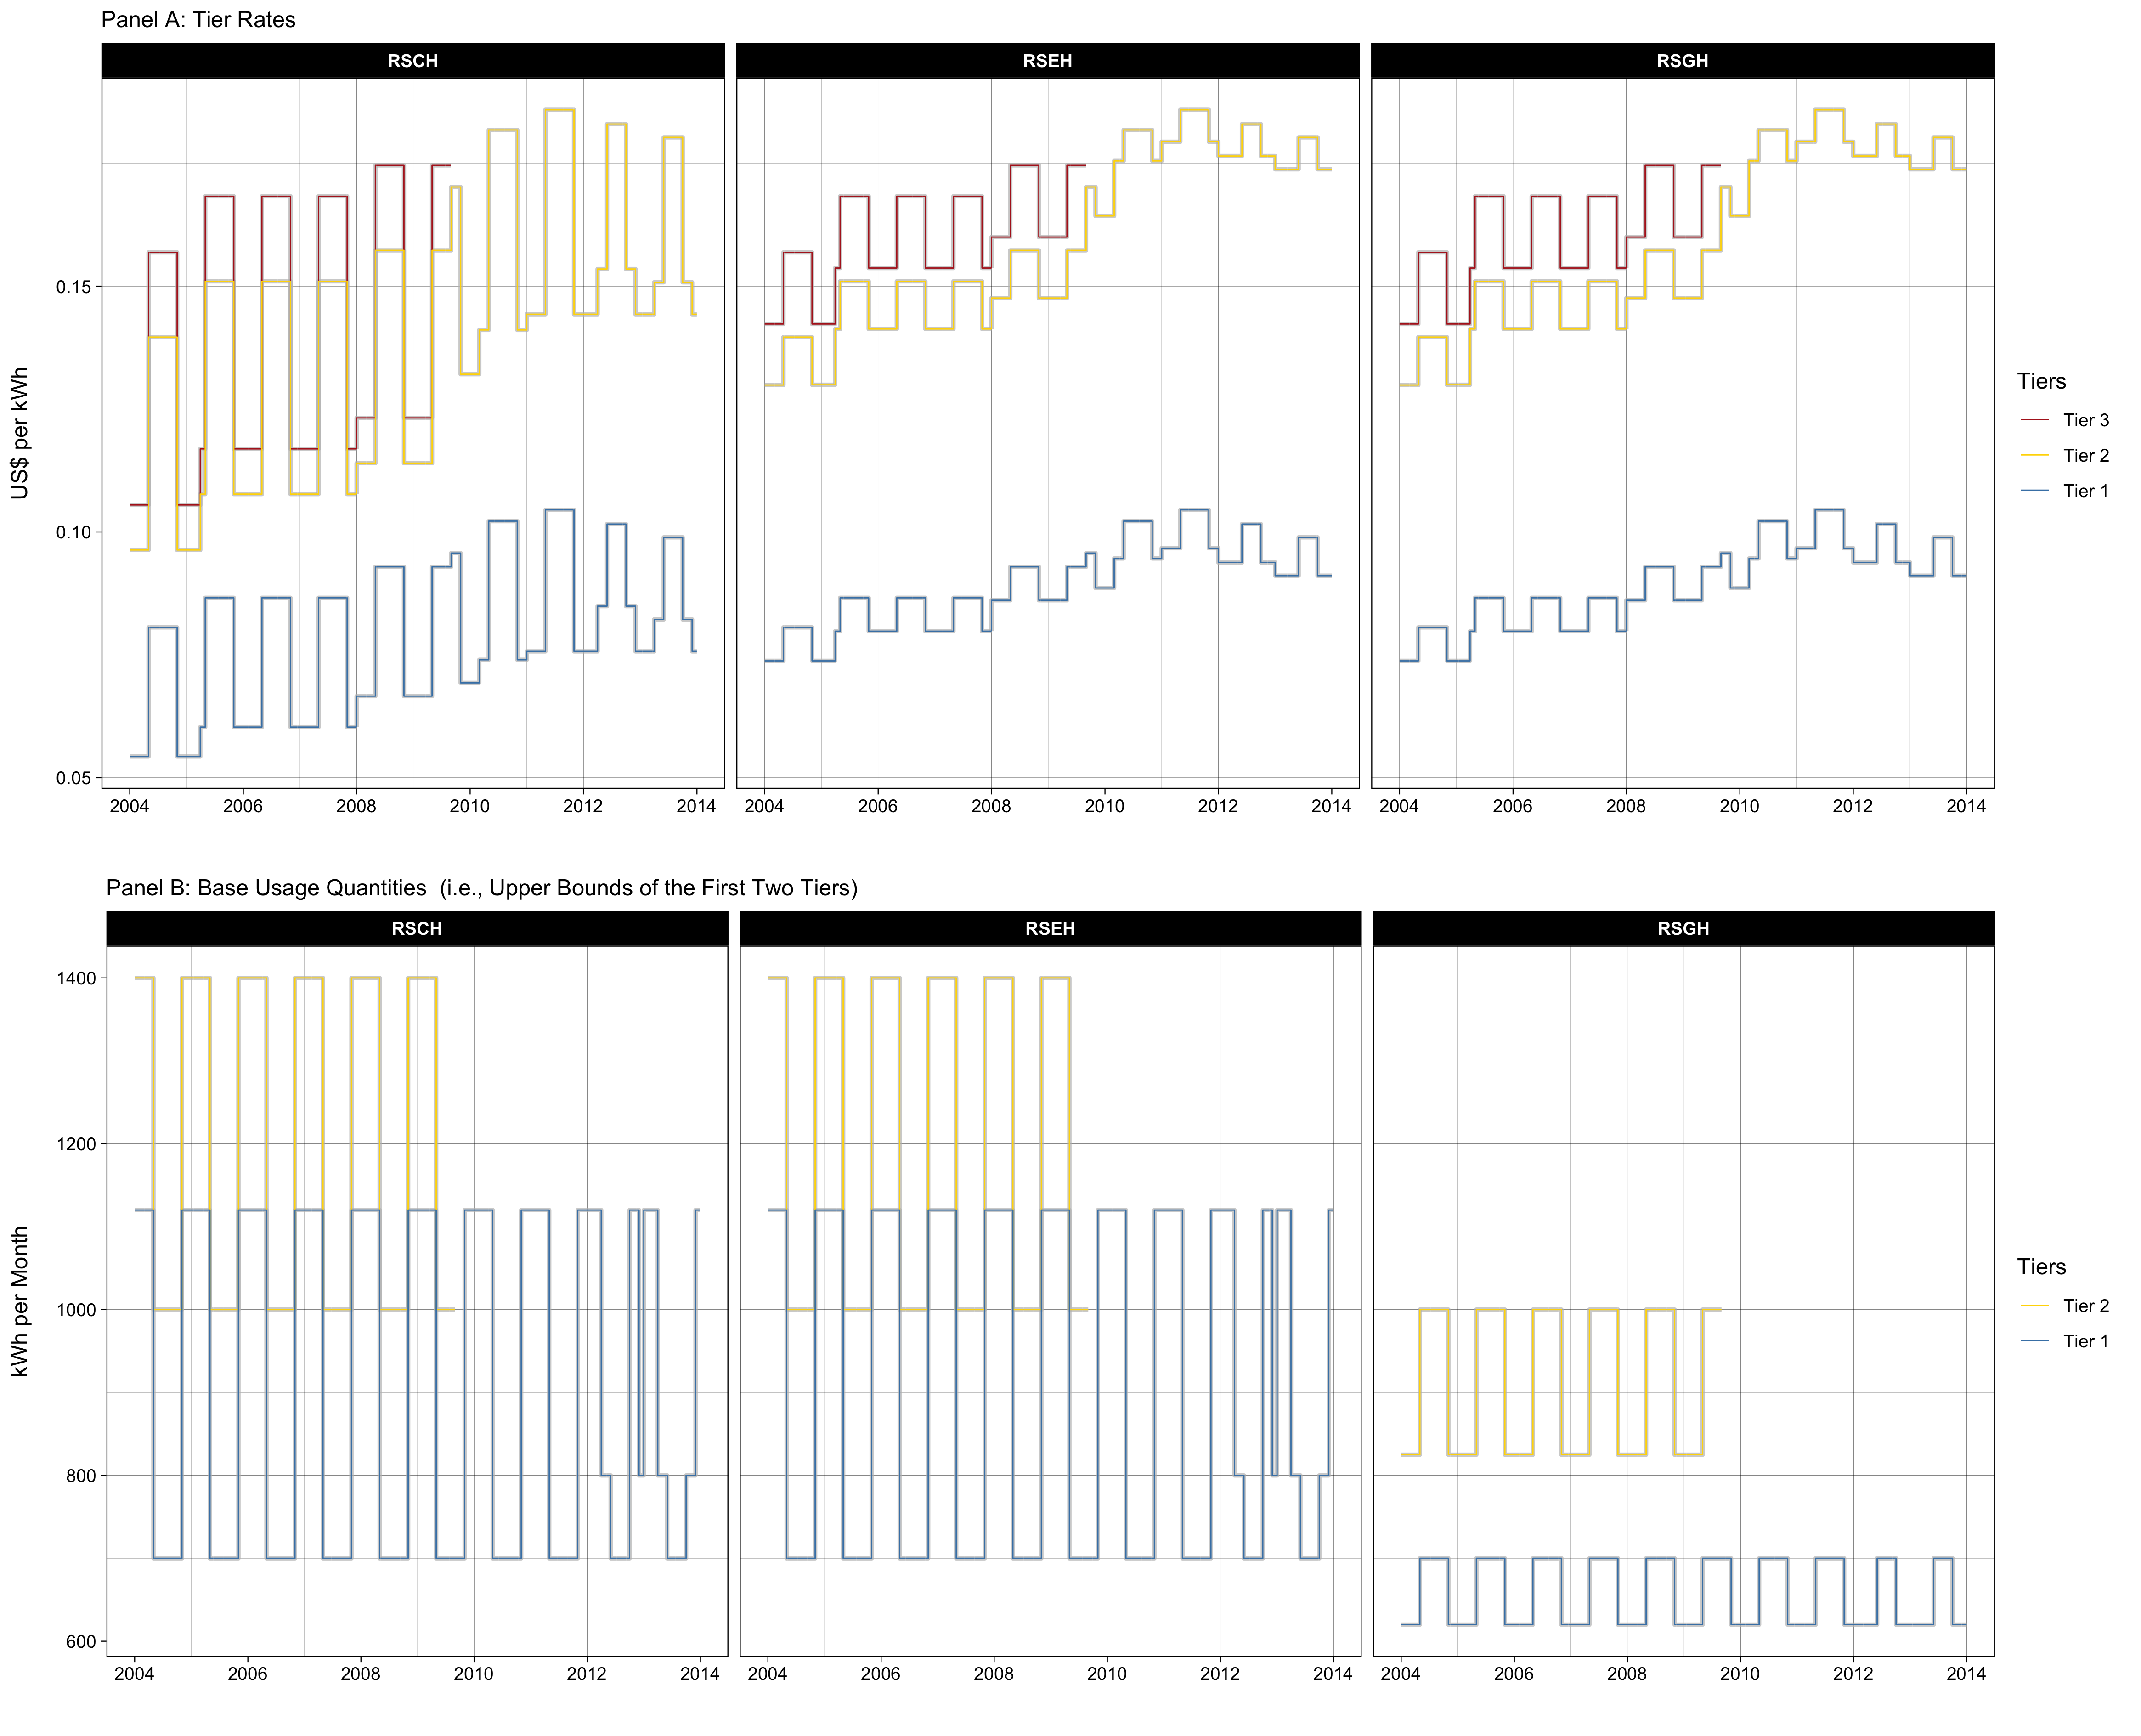
\includegraphics[scale = 0.105]{02_Chapter-1/00A_Figures/Figure_SMUD-Residential-Rates_Variable-Charges-and-Base-Usage-Quantities.png}
        \caption{Tier Rates and Base Usage Quantities of SMUD Residential Rates}
        \subcaption*{
            \textit{Note}: 
            The figure illustrates how SMUD changed tier rates and base usage quantities of the three major residential rates (i.e., RSCH, RSEH, and RSGH) over time. Both tier rates and base usage quantities of the residential rates show significant seasonality. RSCH and RSEH residential rates had the same base usage quantities. There have been only two tiers since September 2009.
        }
        \label{Figure:SMUD-Residential-Rates_Variable-Charge-and-Base-Usage}
    \end{figure}
}
\clearpage

\afterpage{
    \begin{figure}[t!]
        \centering
        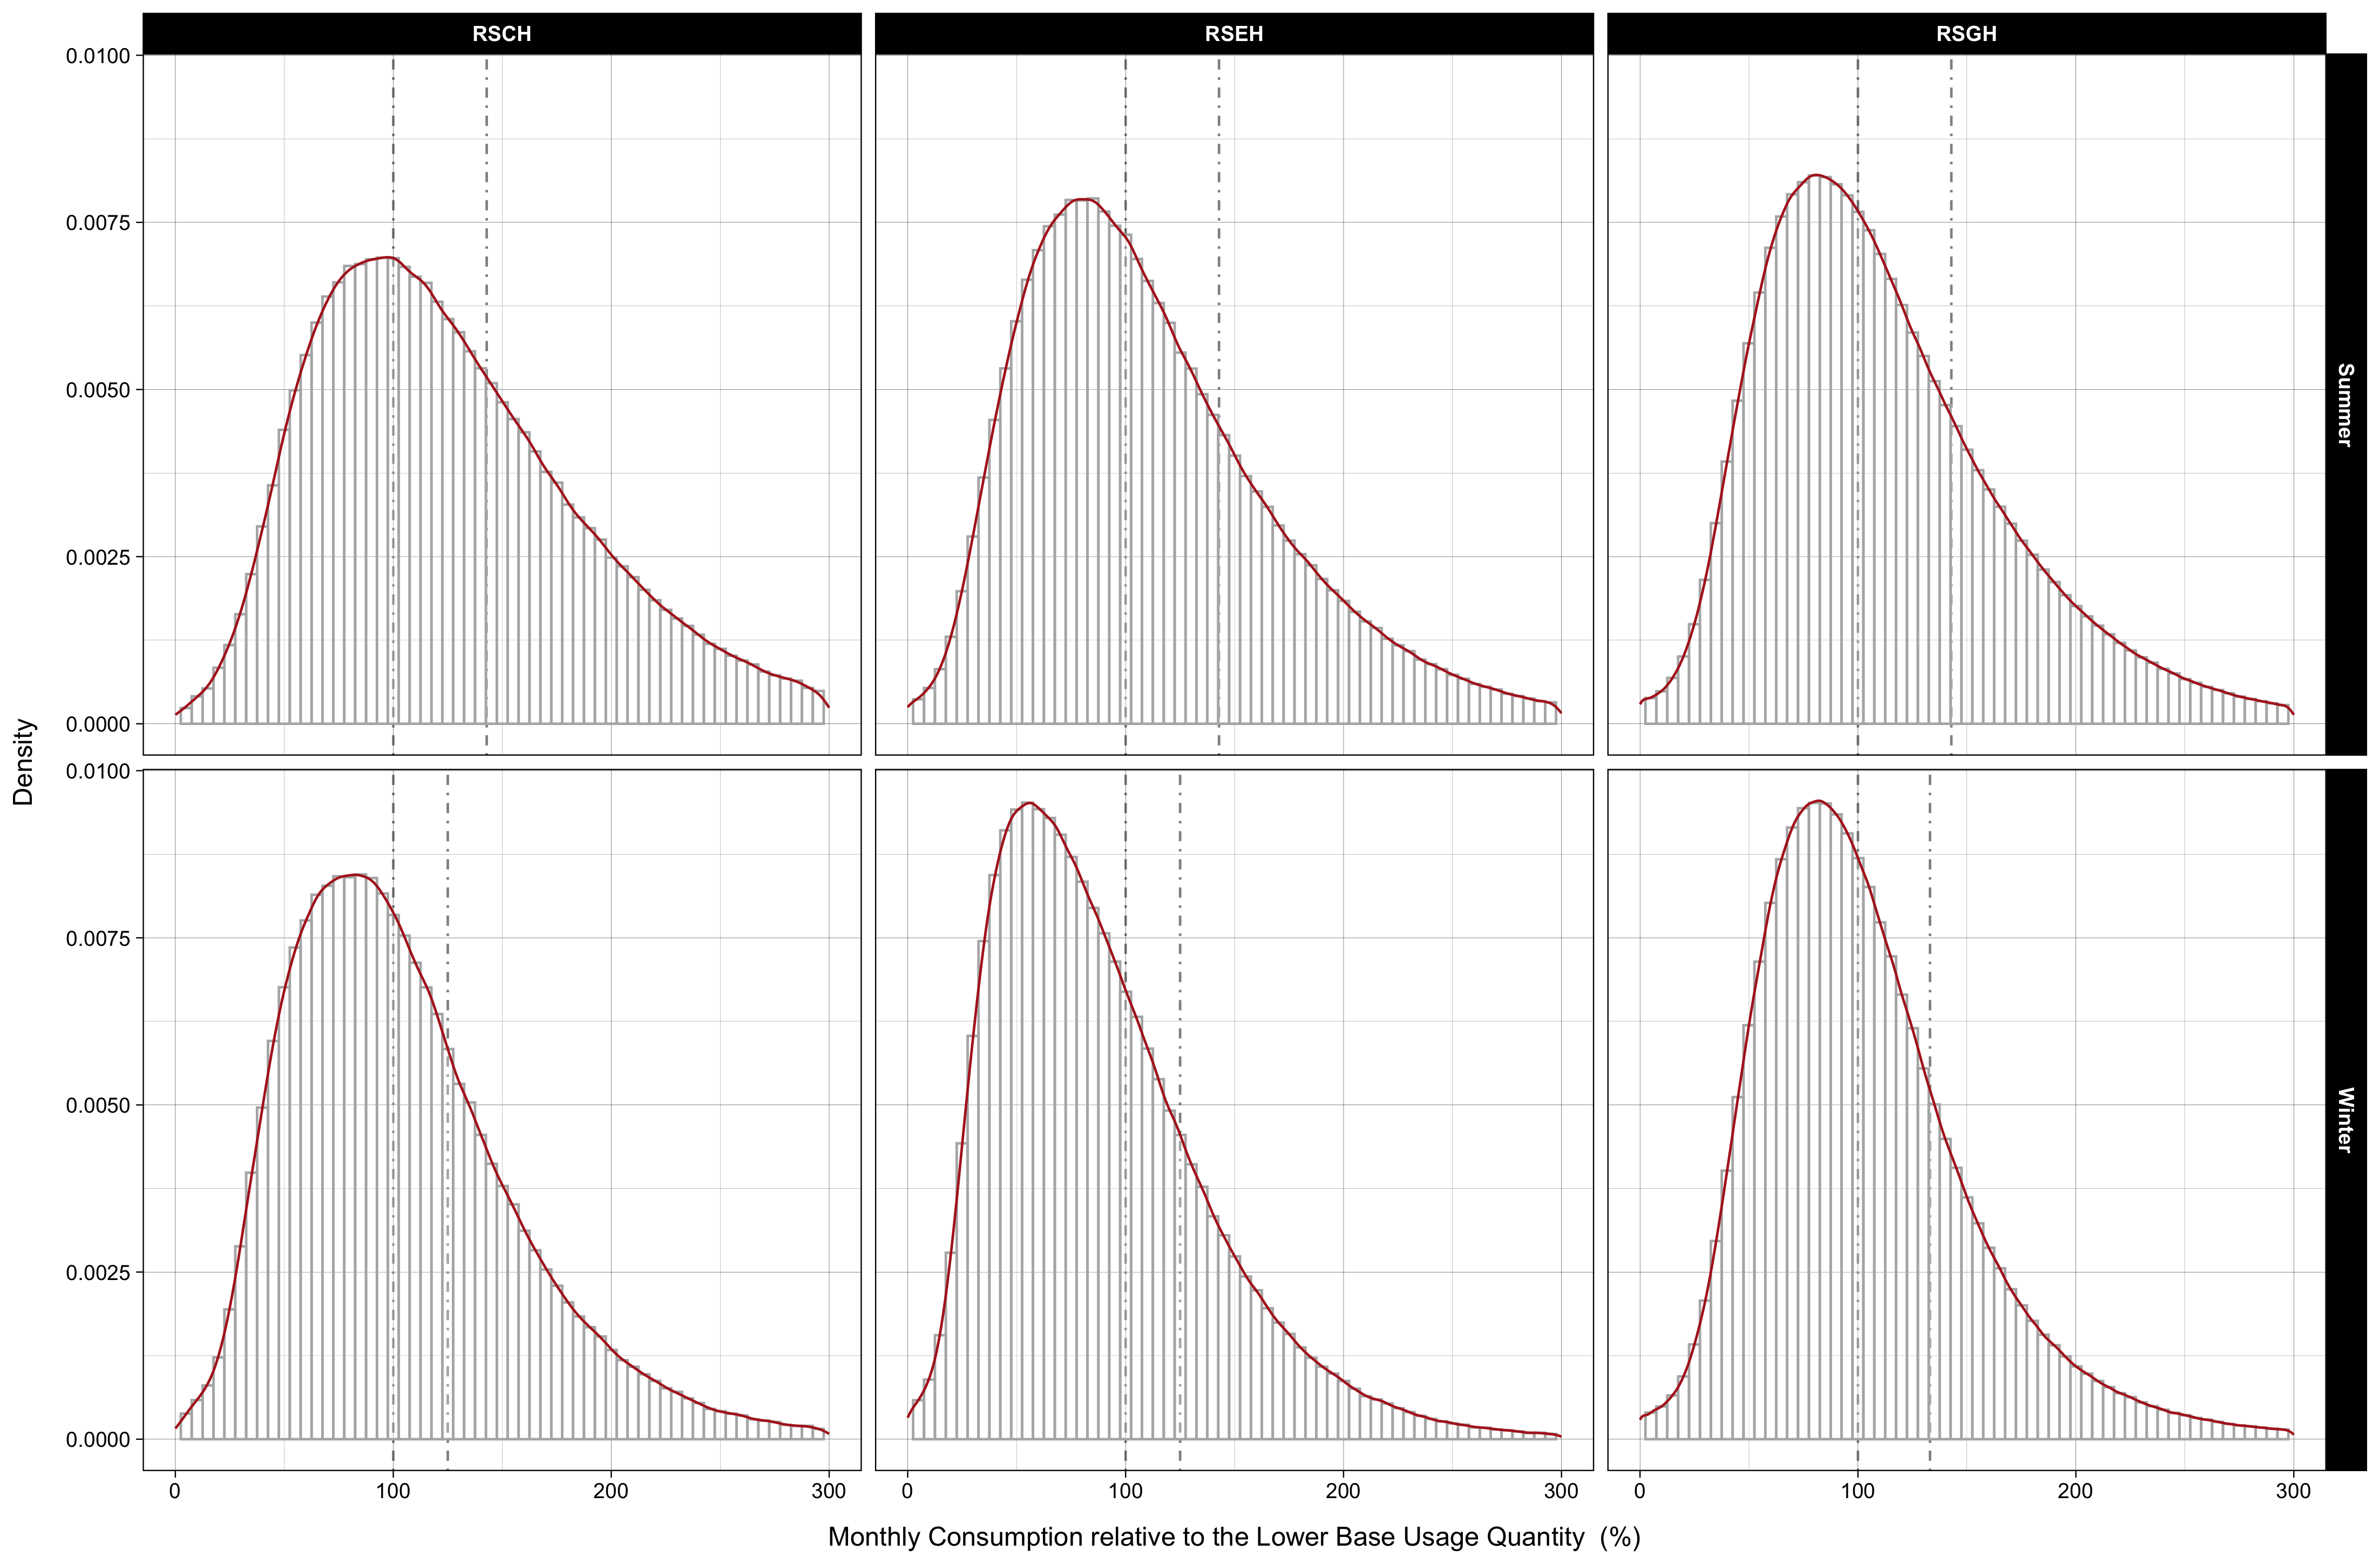
\includegraphics[scale = 0.107]{02_Chapter-1/00A_Figures/Figure_Distribution-of-Electricity-Consumption.png}
        \caption{Distribution of Electricity Consumption by SMUD Residential Customers}
        \subcaption*{
            \textit{Note}: 
            This figure presents histograms---with kernel density estimates---of electricity consumption by SMUD residential customers. Each of the six panels in the figure is for a pair of three major residential rates (i.e., RSCH, RSEH, and RSGH) and two seasons (i.e., summer and winter). Dot-dashed vertical lines in each panel are base usage quantities for the corresponding rate code and season.
        }
        \label{Figure:SMUD-Billing-Data_Histogram_By-Season-and-Rate-Code}
    \end{figure}
}
\clearpage

\afterpage{
    \begin{figure}[t!]
        \centering
        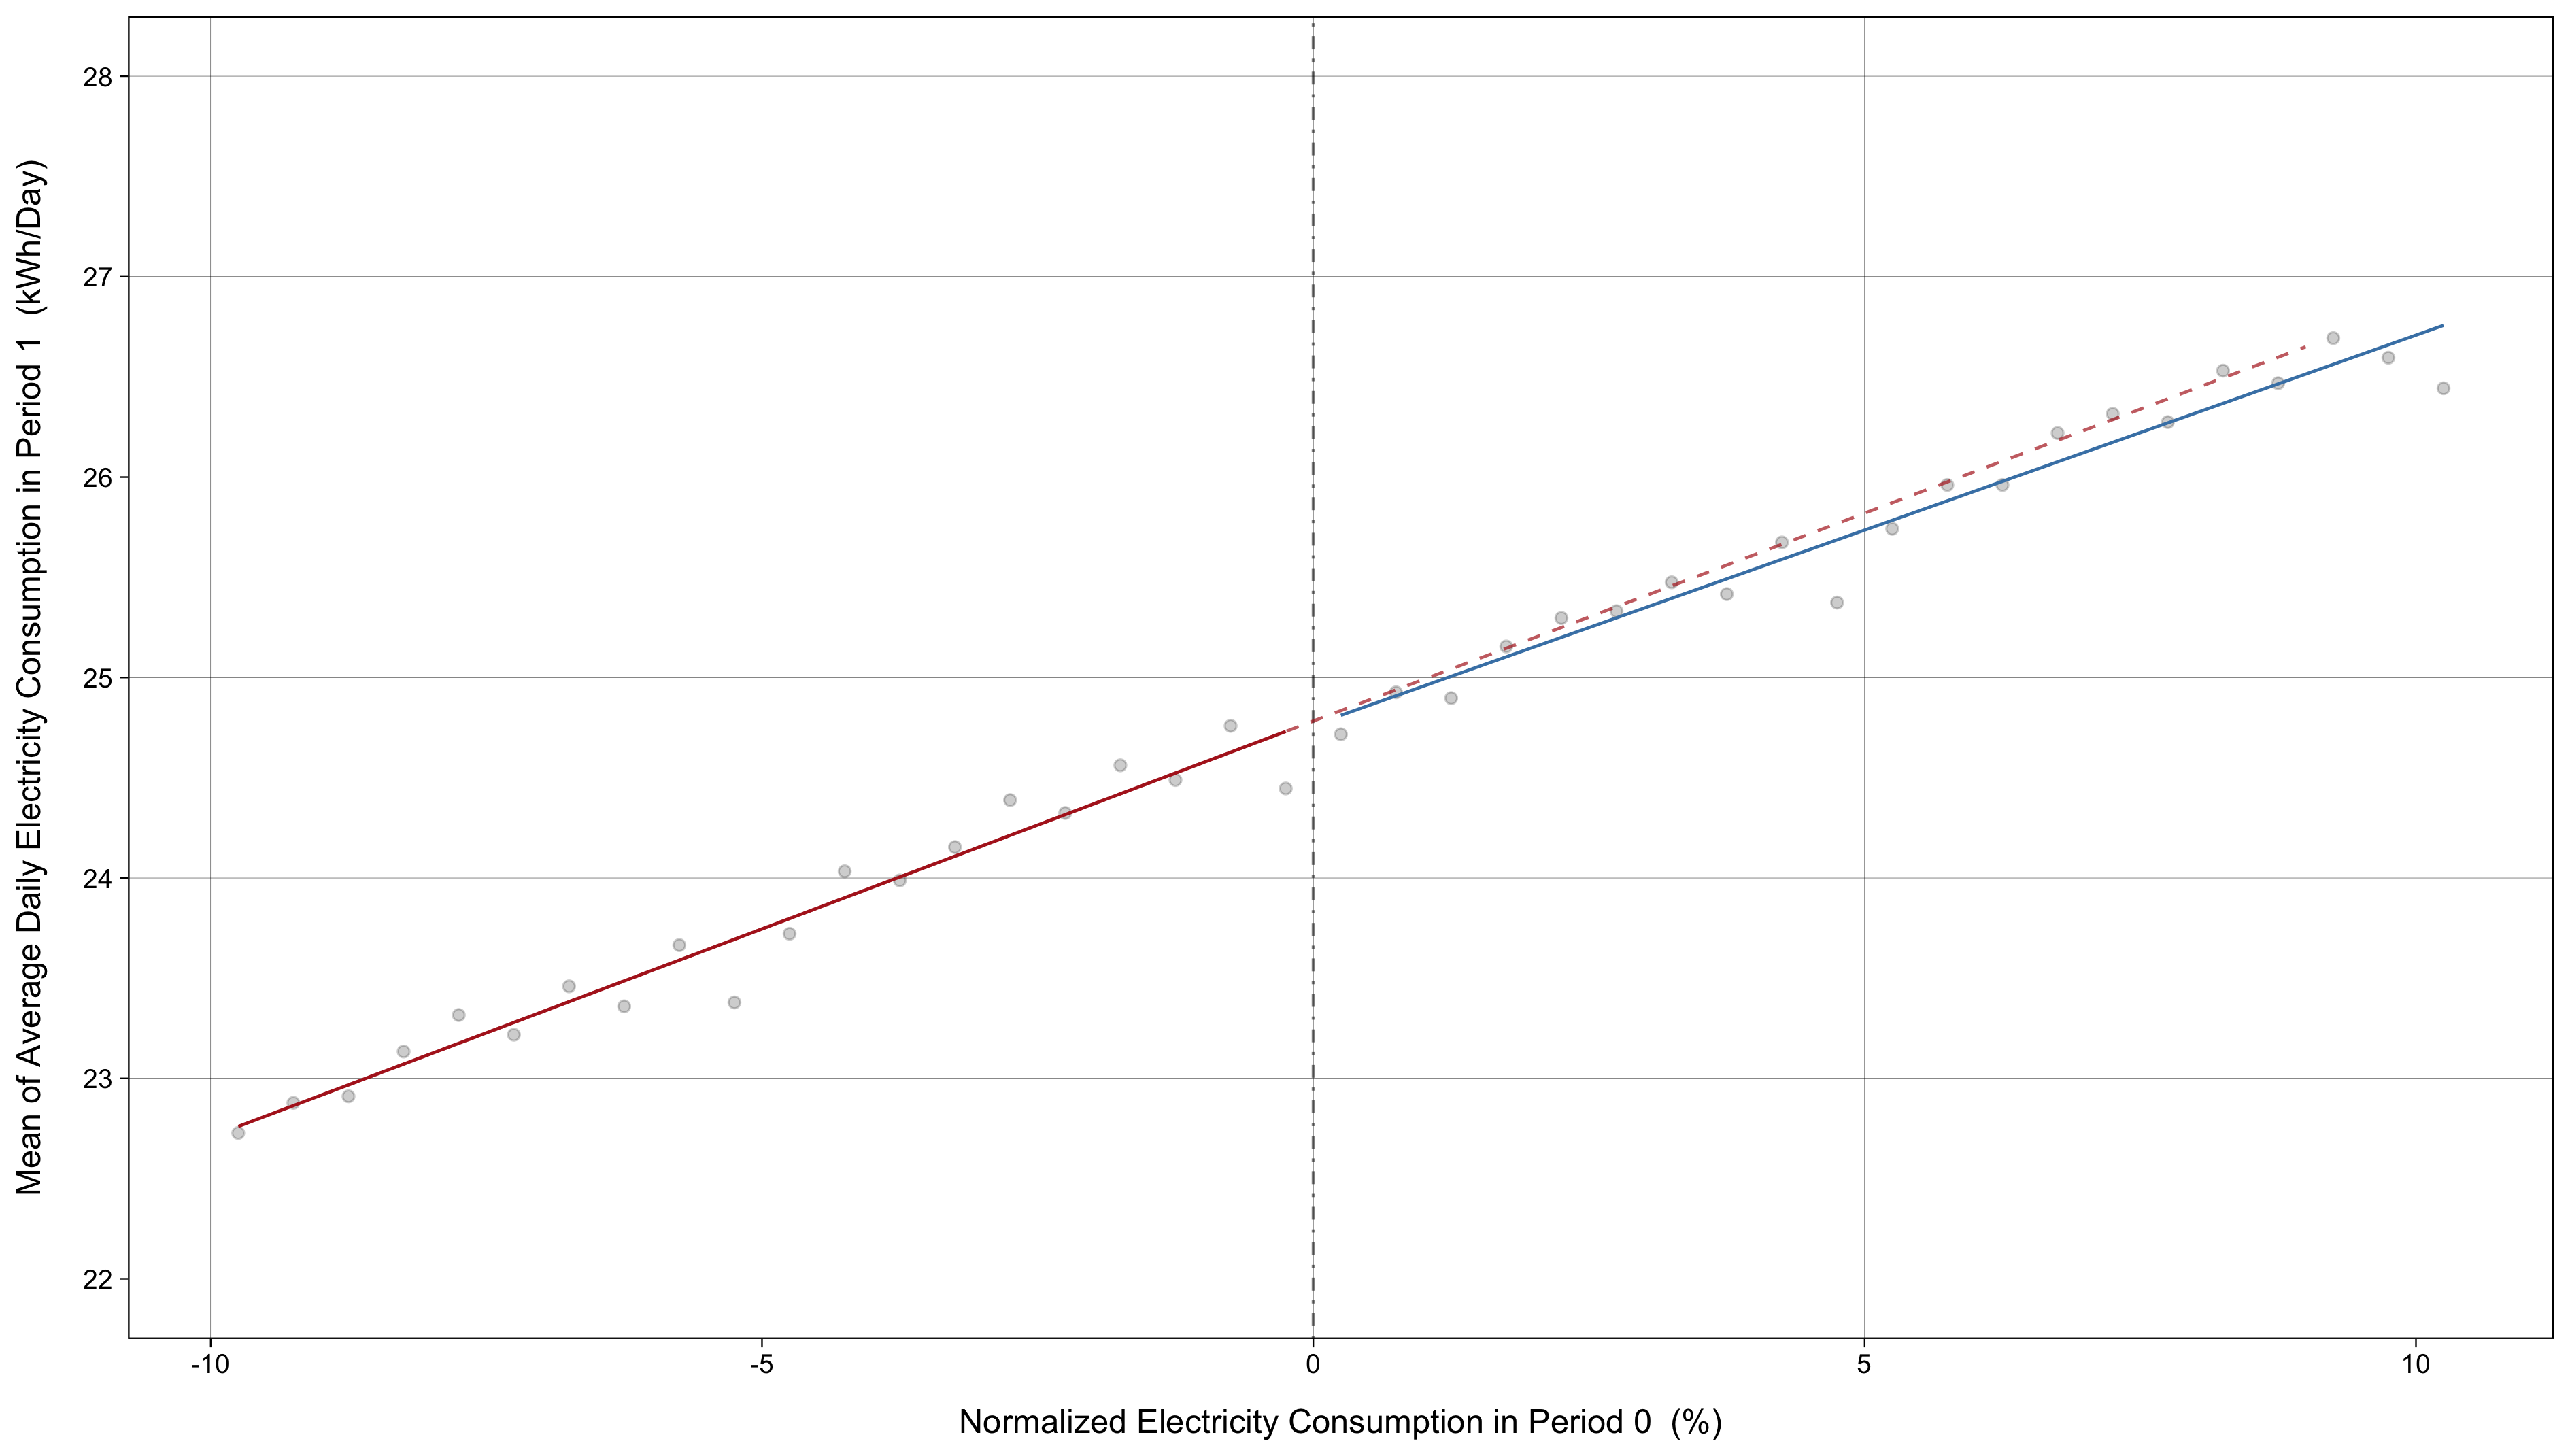
\includegraphics[scale = 0.115]{02_Chapter-1/00A_Figures/Figure_Average-Daily-Electricity-Consumption-in-Period-1-over-NC0.png}
        \caption{Mean of Average Daily Electricity Consumption in Period 1 over $\overline{NC}_{0}$}
        \subcaption*{
            \textit{Note}: 
            ...
        }
        \label{Figure:Average-Daily-Electricity-Consumption-in-Period-1-over-NC0}
    \end{figure}
}
\clearpage

\afterpage{
    \begin{figure}[t!]
        \centering
        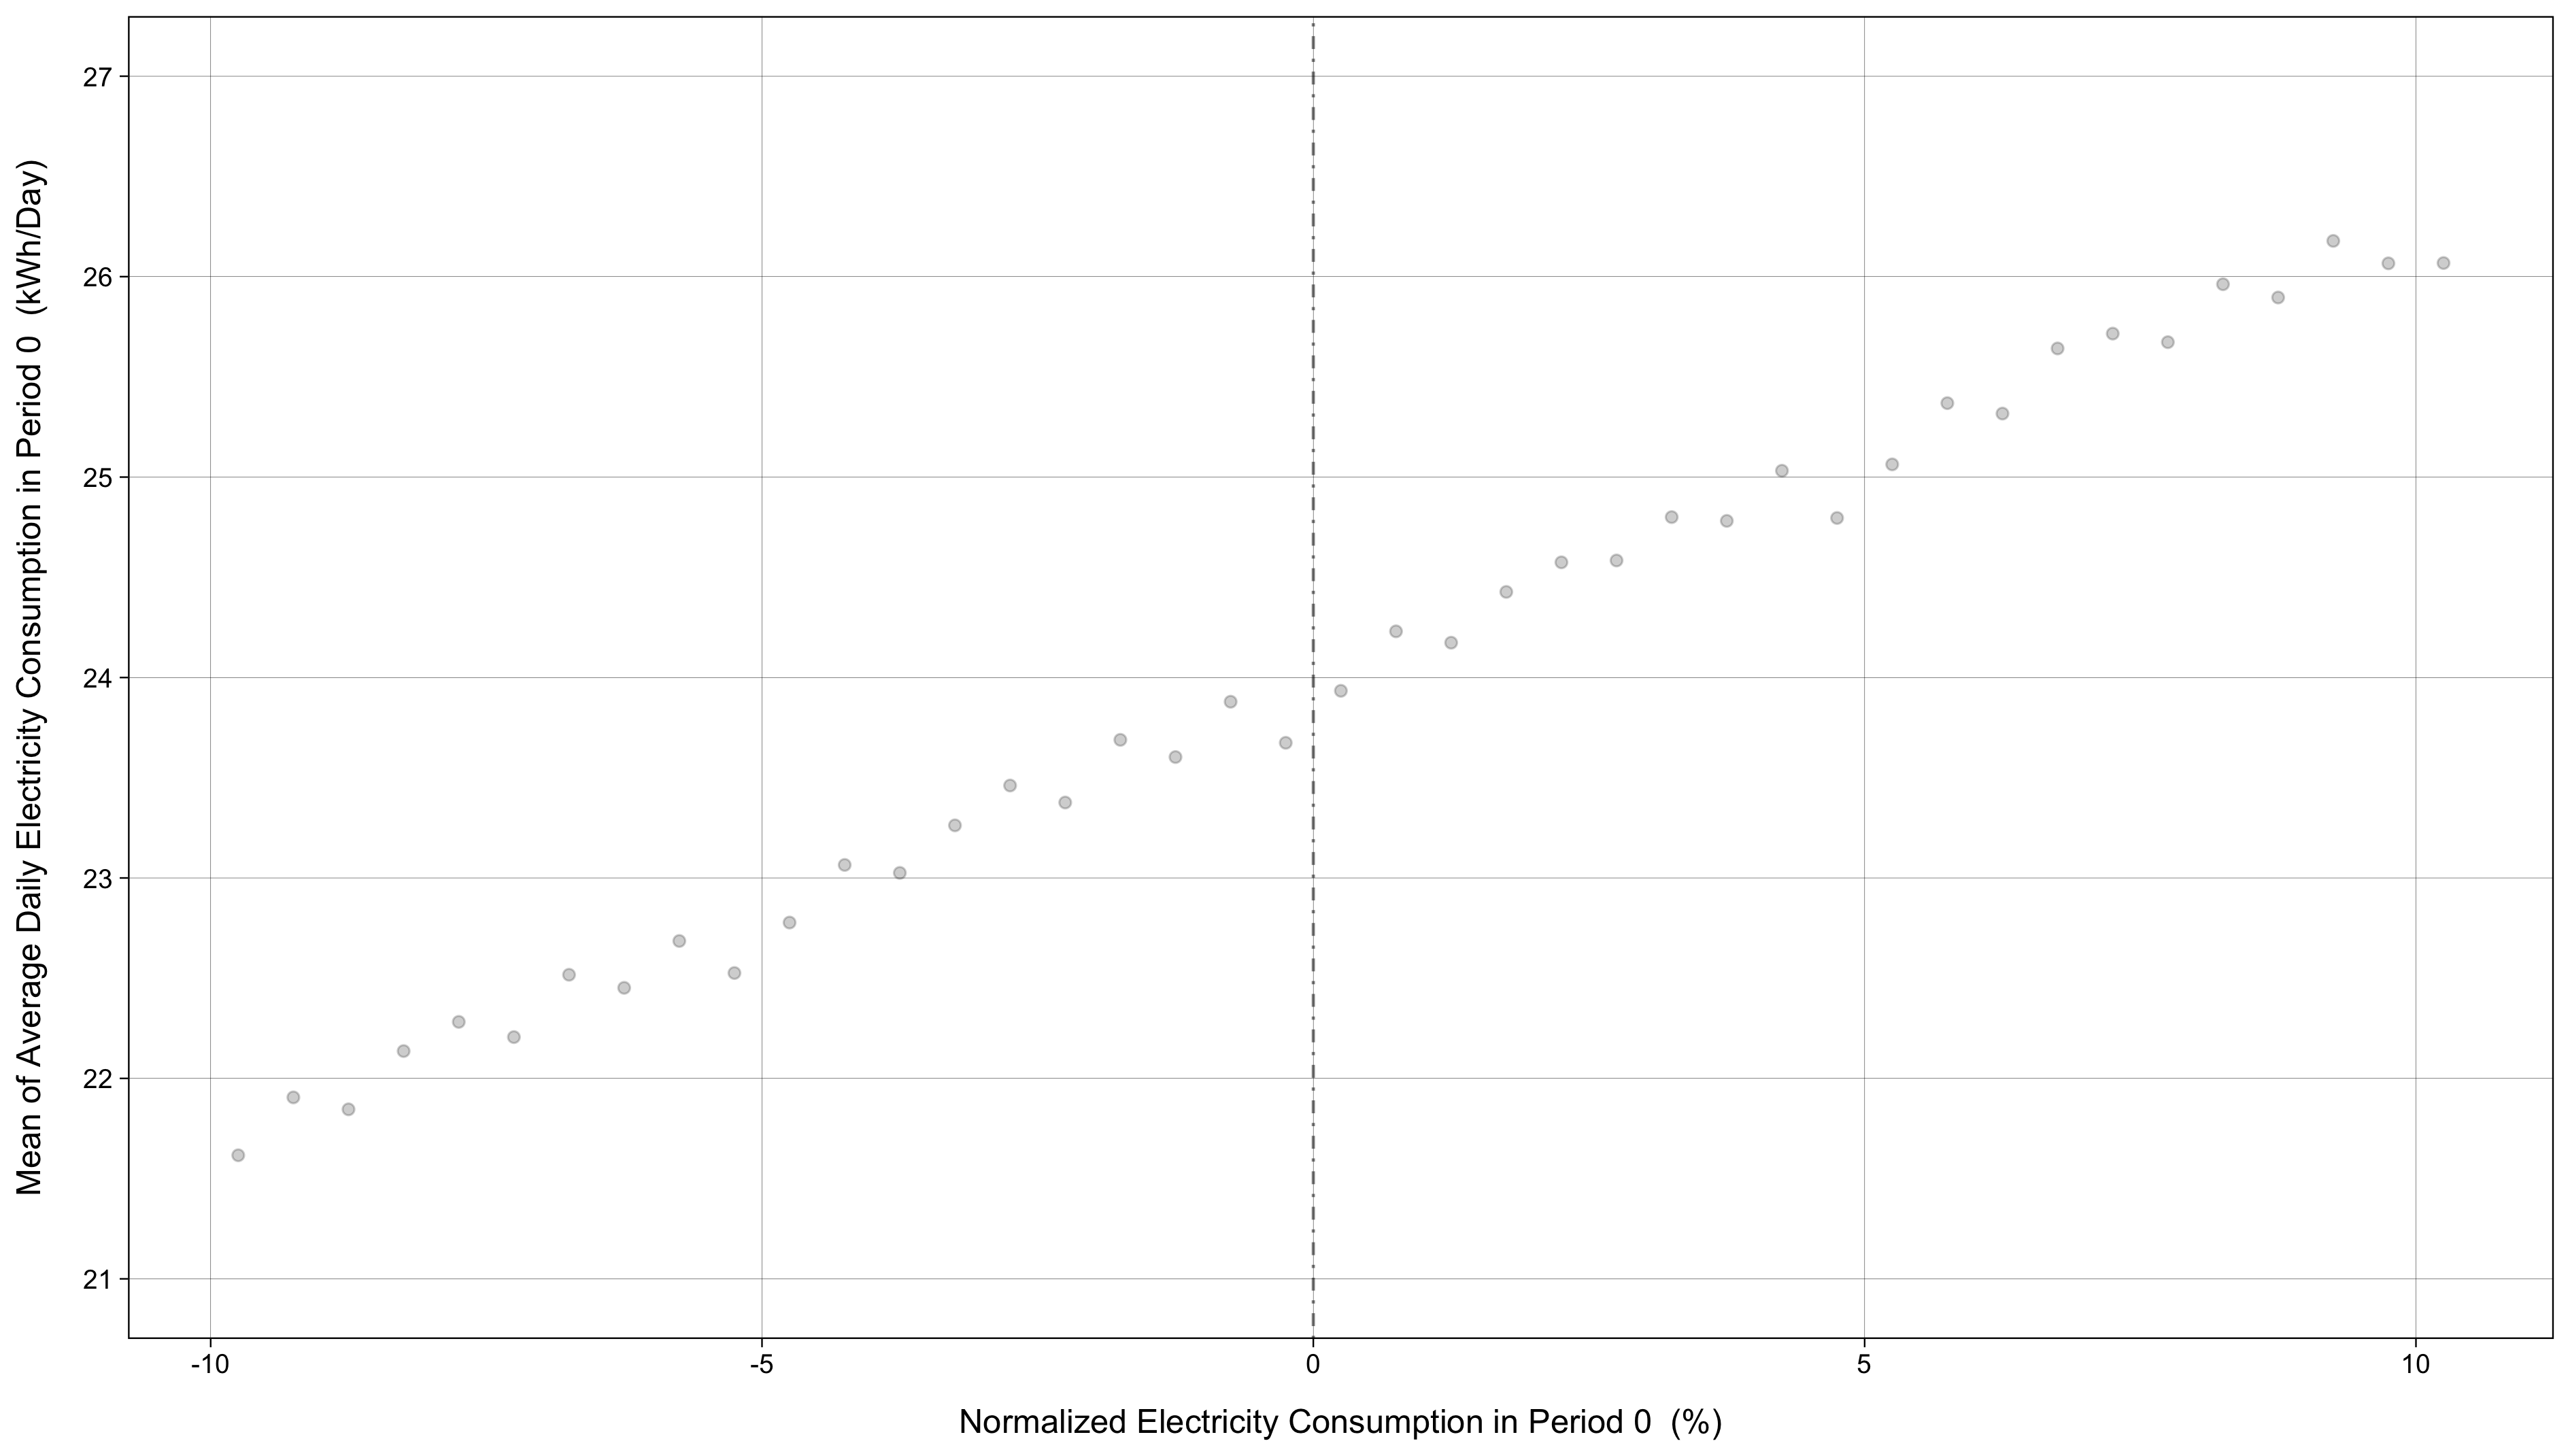
\includegraphics[scale = 0.115]{02_Chapter-1/00A_Figures/Figure_Average-Daily-Electricity-Consumption-in-Period-0-over-NC0.png}
        \caption{Mean of Average Daily Electricity Consumption in Period 0 over $\overline{NC}_{0}$}
        \subcaption*{
            \textit{Note}: 
            ...
        }
        \label{Figure:Average-Daily-Electricity-Consumption-in-Period-0-over-NC0}
    \end{figure}
}
\clearpage

\afterpage{
    \begin{figure}[t!]
        \centering
        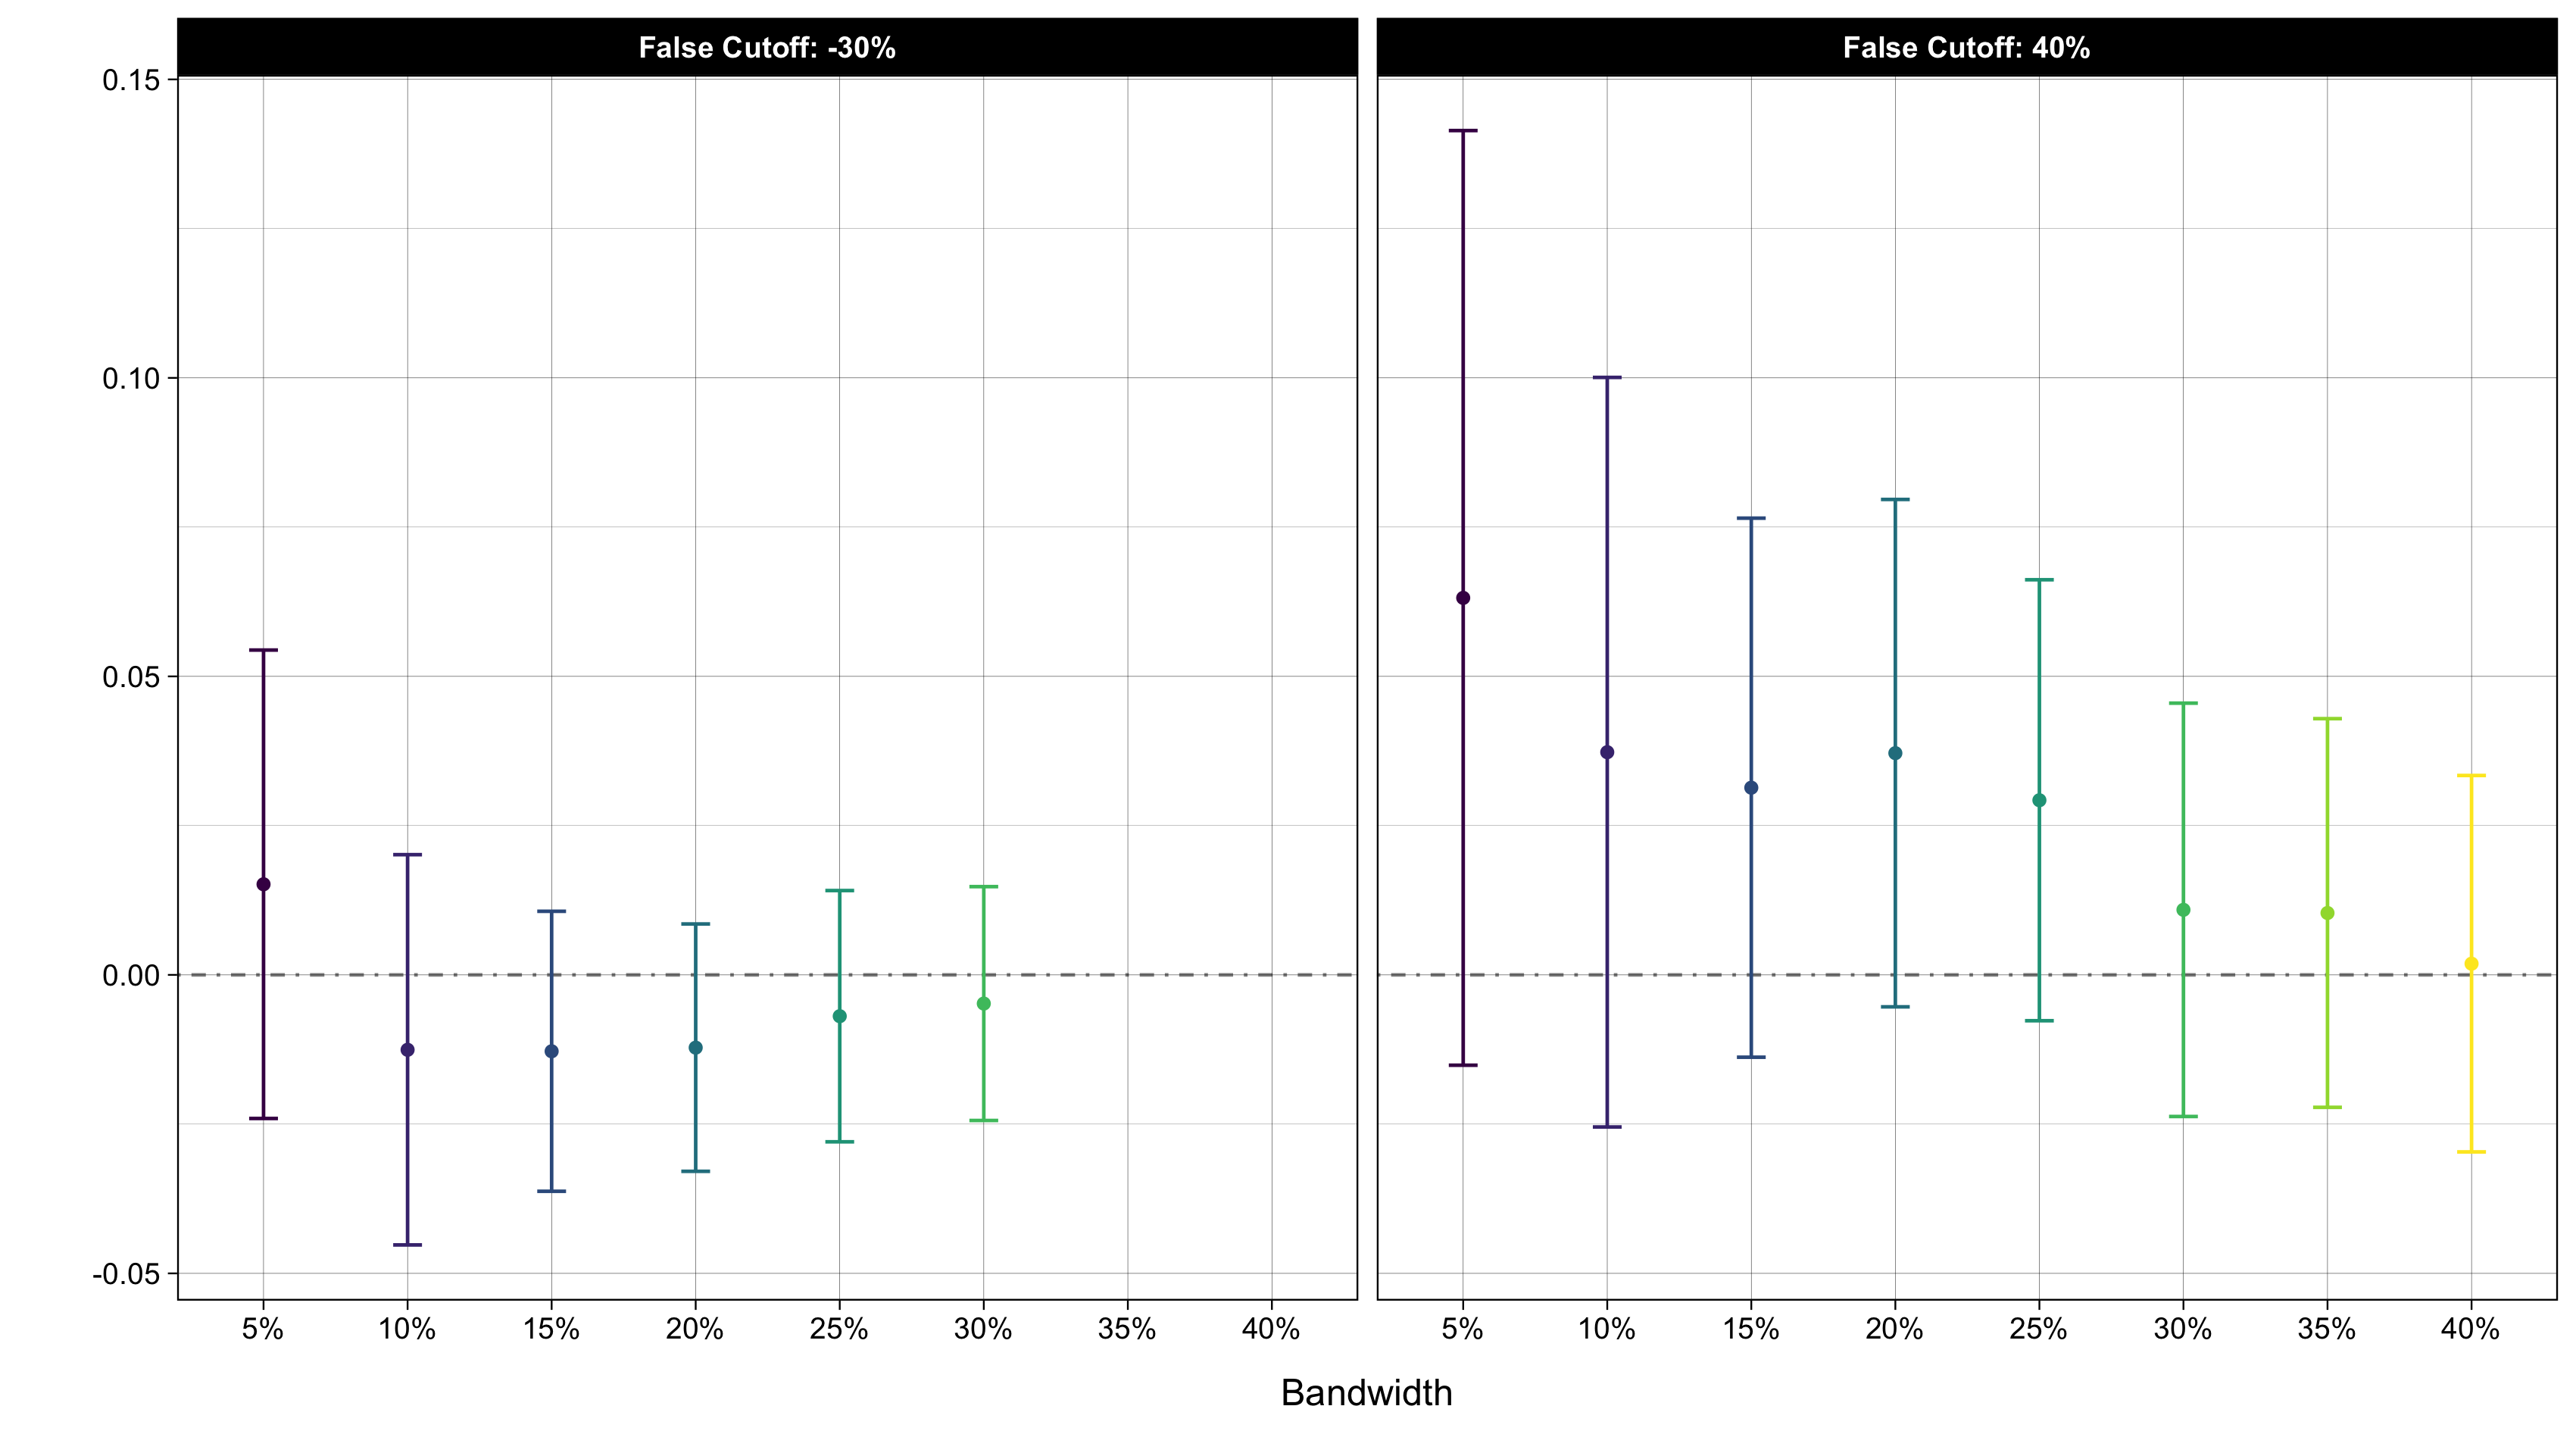
\includegraphics[scale = 0.14]{02_Chapter-1/00A_Figures/Figure_Falsification-Tests_With-False-Cutoff-40-and-M30.png}
        \caption{Robustness Checks: Falsification Tests}
        \subcaption*{
            \textit{Note}: 
            ...
        }
        \label{Figure:Robustness-Checks_Falsification-Tests}
    \end{figure}
}
\clearpage

\afterpage{
    \begin{figure}[t!]
        \centering
        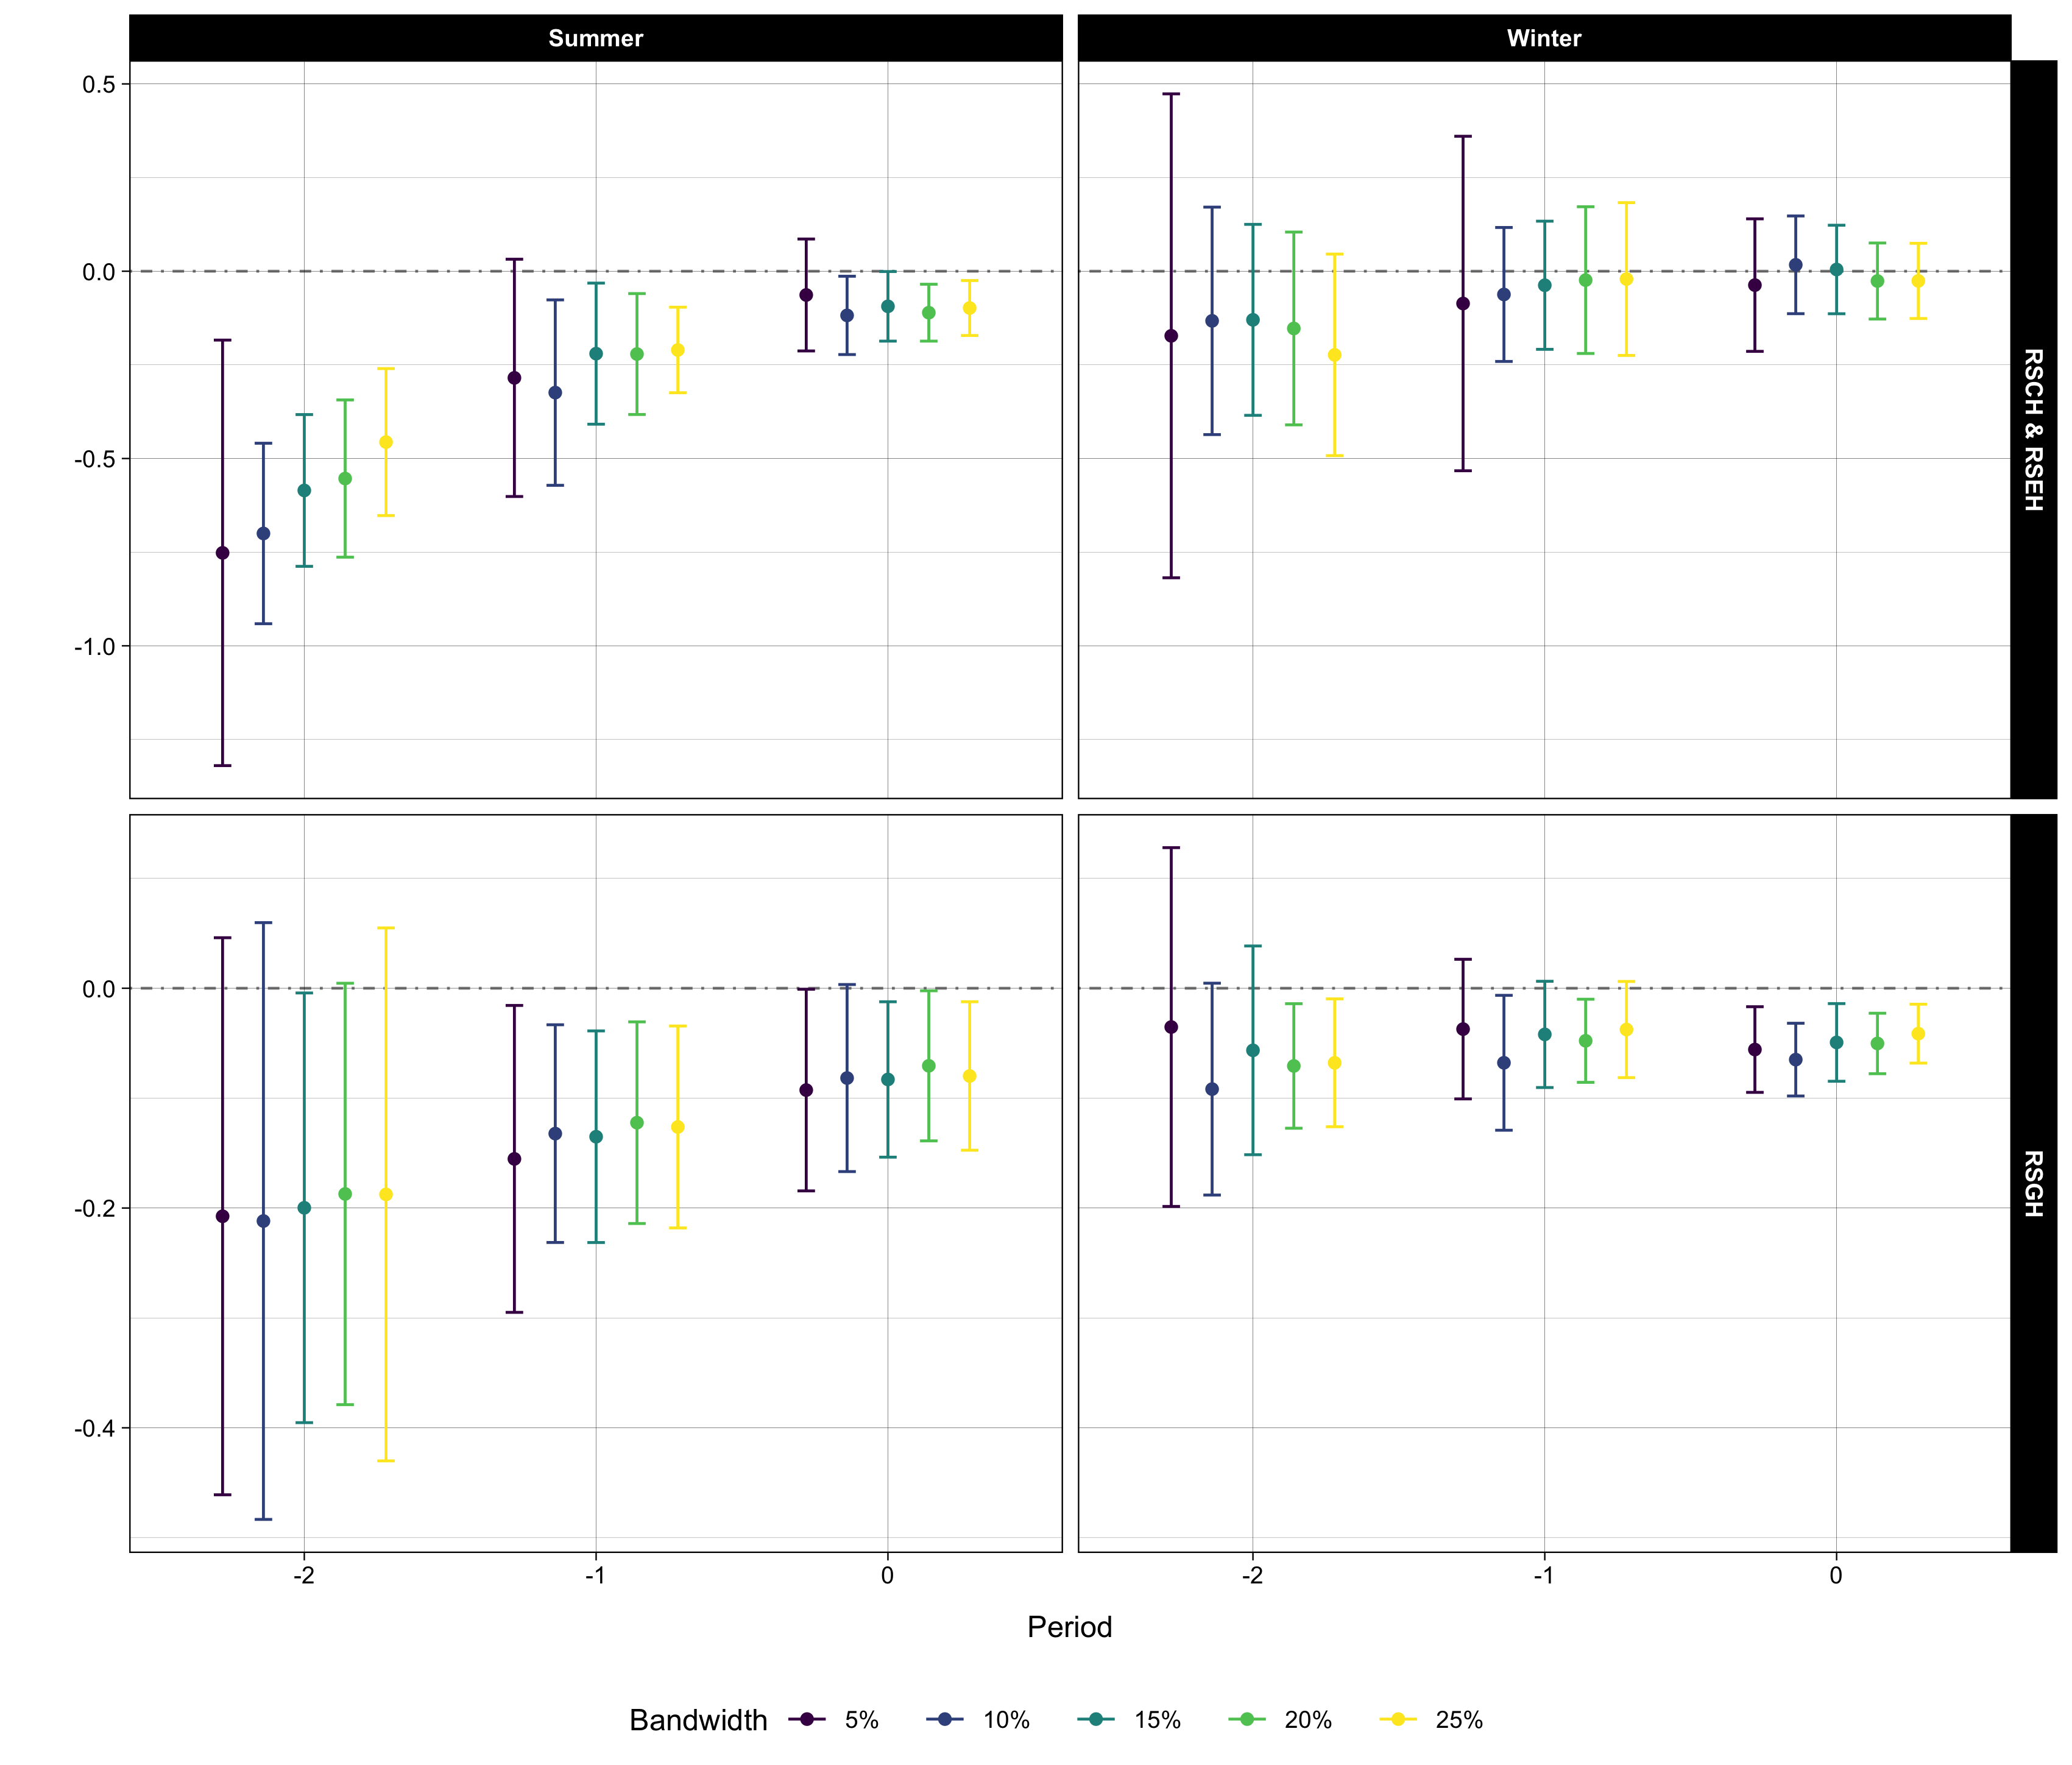
\includegraphics[scale = 0.135]{02_Chapter-1/00A_Figures/Figure_Multi-Period-Treatment-Effects_By-Season.png}
        \caption{Multi-Period Treatment Effects}
        \subcaption*{
            \textit{Note}: 
            ... 
        }
        \label{Figure:Multi-Period-Treatment-Effects}
    \end{figure}
}
\clearpage



% Tables
\setcounter{table}{1}
\afterpage{
    \begin{table}[t!]
        \centering
        \caption{Summary Statistics}
        \label{Table:Summary-Statistics}
        \vspace{0.3cm}
        \small
        \begin{adjustbox}{scale = 1.0}
            \begin{tabular}{
                >{\raggedright}m{2.0cm}
                >{\raggedleft}m{2.5cm}
                >{\raggedleft}m{3.0cm}
                >{\raggedleft}m{1.7cm}
                >{\raggedleft}m{1.7cm}
                >{\raggedleft}m{1.7cm}
                >{\raggedleft\arraybackslash}m{1.7cm}
            }
                \hline \hline
                \multicolumn{1}{c}{Bandwidth} & \multicolumn{1}{c}{Households} & \multicolumn{1}{c}{Observations} & \multicolumn{2}{c}{Control} & \multicolumn{2}{c}{Treatment} \\
                \cline{4-5} \cline{6-7}
                \multicolumn{1}{c}{} & \multicolumn{1}{c}{} & \multicolumn{1}{c}{} & \multicolumn{1}{c}{Mean} & \multicolumn{1}{c}{(S.D.)} & \multicolumn{1}{c}{Mean} & \multicolumn{1}{c}{(S.D.)} \\
                \hline
                \underline{Normalized Electricity Consumption in Period 0 \ (\%)} & & & & & & \\
                \hspace{0.55cm} 5\% & $286,671$ & $1,186,630$ & $-2.454$ & $1.444$ & $2.485$ & $1.407$ \\
                \hspace{0.55cm} 10\% & $318,880$ & $2,378,864$ & $-4.993$ & $2.885$ & $4.918$ & $2.847$ \\
                \hspace{0.55cm} 15\% & $331,605$ & $3,566,318$ & $-7.543$ & $4.324$ & $7.357$ & $4.322$ \\
                \hspace{0.55cm} 20\% & $338,470$ & $4,702,081$ & $-10.085$ & $5.756$ & $9.617$ & $5.718$ \\
                \hspace{0.55cm} 25\% & $343,139$ & $5,816,854$ & $-12.612$ & $7.184$ & $11.870$ & $7.144$ \\
                \hspace{0.55cm} 30\% & $341,917$ & $6,276,579$ & $-15.054$ & $8.597$ & $14.063$ & $8.559$ \\
                & & & & & & \\
                \underline{Average Daily Electricity Consumption in Period 1 \ ($kWh/Day$)} & & & & & & \\
                \hspace{0.55cm} 5\% & $286,671$ & $1,186,630$ & $24.329$ & $7.922$ & $25.296$ & $8.143$ \\ 
                \hspace{0.55cm} 10\% & $318,880$ & $2,378,864$ & $23.776$ & $7.786$ & $25.782$ & $8.290$ \\
                \hspace{0.55cm} 15\% & $331,605$ & $3,566,318$ & $23.231$ & $7.674$ & $26.270$ & $8.450$ \\
                \hspace{0.55cm} 20\% & $338,470$ & $4,702,081$ & $22.681$ & $7.582$ & $26.744$ & $8.624$ \\
                \hspace{0.55cm} 25\% & $343,139$ & $5,816,854$ & $22.140$ & $7.509$ & $27.202$ & $8.805$ \\
                \hspace{0.55cm} 30\% & $341,917$ & $6,276,579$ & $20.674$ & $6.560$ & $26.517$ & $7.874$ \\ 
                \hline \hline
            \end{tabular}
        \end{adjustbox}
        \begin{tablenotes}[flushleft]
            \footnotesize
            \item \textit{Note}: This table presents summary statistics for household electricity consumption. 
        \end{tablenotes}
    \end{table}
}

\clearpage

\afterpage{
    \begin{table}[t!]
        \centering
        \caption{Regression Discontinuity Results}
        \label{Table:RD-Results}
        \vspace{0.3cm}
        \small
        \begin{adjustbox}{scale = 0.8}
            \begin{threeparttable}
                \begin{tabular}{@{\extracolsep{-1.5pt}}lcccccccccc}
                    \\[-5.5ex]
                    \hline \hline
                    \\[-3.0ex]
                    & \multicolumn{10}{c}{Dependent Variable} \\
                    \\[-3.0ex]
                    \cline{2-11}
                    \\[-3.0ex]
                    & \multicolumn{10}{c}{Average Daily Electricity Consumption  (kWh/Day)} \\
                    \\[-3.0ex]
                    & (1) & (2) & (3) & (4) & (5) & (6) & (7) & (8) & (9) & (10) \\
                    \\[-3.0ex]
                    \hline
                    \\[-2.0ex]
                    $\mathbb{1}$[Treatment] & $-$0.080$^{***}$ & $-$0.089$^{***}$ & $-$0.012 & $-$0.071$^{***}$ & $-$0.024$^{**}$ & $-$0.075$^{***}$ & $-$0.084$^{***}$ & $-$0.014 & $-$0.066$^{***}$ & $-$0.021$^{*}$ \\
                    & (0.022) & (0.026) & (0.012) & (0.014) & (0.011) & (0.022) & (0.026) & (0.012) & (0.014) & (0.011) \\
                    & & & & & & & & & & \\
                    NC0 & 0.209$^{***}$ & 0.200$^{***}$ & 0.088$^{***}$ & 0.221$^{***}$ & 0.134$^{***}$ & 0.212$^{***}$ & 0.204$^{***}$ & 0.086$^{***}$ & 0.225$^{***}$ & 0.136$^{***}$ \\
                    & (0.006) & (0.005) & (0.005) & (0.005) & (0.006) & (0.006) & (0.006) & (0.005) & (0.005) & (0.006) \\
                    & & & & & & & & & & \\
                    $\mathbb{1}$[Treatment] $\times$ NC0 &  &  &  &  &  & $-$0.007$^{***}$ & $-$0.008$^{***}$ & 0.004$^{*}$ & $-$0.008$^{***}$ & $-$0.004$^{**}$ \\
                    &  &  &  &  &  & (0.002) & (0.002) & (0.002) & (0.002) & (0.002) \\
                    & & & & & & & & & & \\
                    Average Daily CDDs &  & 0.791$^{***}$ & 1.100$^{***}$ & 1.164$^{***}$ & 1.206$^{***}$ &  & 0.791$^{***}$ & 1.100$^{***}$ & 1.164$^{***}$ & 1.206$^{***}$ \\
                    &  & (0.116) & (0.066) & (0.100) & (0.055) &  & (0.116) & (0.066) & (0.100) & (0.055) \\
                    & & & & & & & & & & \\
                    Average Daily HDDs &  & 0.327$^{***}$ & 0.432$^{***}$ & 0.507$^{***}$ & 0.492$^{***}$ &  & 0.327$^{***}$ & 0.432$^{***}$ & 0.507$^{***}$ & 0.492$^{***}$ \\
                    &  & (0.073) & (0.039) & (0.106) & (0.051) &  & (0.073) & (0.039) & (0.106) & (0.051) \\
                    & & & & & & & & & & \\
                    (Constant) & 24.756$^{***}$ & 19.472$^{***}$ &  &  &  & 24.789$^{***}$ & 19.508$^{***}$ &  &  &  \\
                    & (0.526) & (0.903) &  &  &  & (0.525) & (0.907) &  &  &  \\
                    & & & & & & & & & & \\
                    \hline
                    \\[-2.0ex]
                    Bandwidth & 20\% & 20\% & 20\% & 20\% & 20\% & 20\% & 20\% & 20\% & 20\% & 20\% \\
                    FEs: Account-by-Premise IDs &  &  & Yes &  & Yes &  &  & Yes &  & Yes \\
                    FEs: Billing Year-by-Month &  &  &  & Yes & Yes &  &  &  & Yes & Yes \\
                    Observations & 5,010,089 & 5,010,089 & 5,010,089 & 5,010,089 & 5,010,089 & 5,010,089 & 5,010,089 & 5,010,089 & 5,010,089 & 5,010,089 \\
                    Adjusted R$^{2}$ & 0.078 & 0.174 & 0.529 & 0.331 & 0.582 & 0.078 & 0.174 & 0.529 & 0.331 & 0.582 \\
                    \\[-2.0ex]
                    \hline \hline
                    \\[-4.5ex]
                \end{tabular}
                \begin{tablenotes}[flushleft]
                    \footnotesize
                    \item \textit{Note}: * $p < 0.1$, ** $p < 0.05$, and *** $p < 0.01$.
                \end{tablenotes}
            \end{threeparttable}
        \end{adjustbox}
    \end{table}
}

\clearpage

\afterpage{
    \begin{table}[t!]
        \centering
        \caption{Robustness Checks: For Different Bandwidths}
        \label{Table:Robustness-Checks_BWs}
        \vspace{0.3cm}
        \footnotesize
        \begin{adjustbox}{scale = 0.85}
            \begin{threeparttable}
                \begin{tabular}{@{\extracolsep{5pt}}lcccccccc}
                    \\[-5.5ex]
                    \hline \hline
                    \\[-3.0ex]
                     & \multicolumn{8}{c}{Dependent Variable} \\
                    \\[-3.0ex]
                    \cline{2-9}
                    \\[-3.0ex]
                     & \multicolumn{8}{c}{Average Daily Electricity Consumption  (kWh/Day)} \\
                    \\[-3.0ex]
                     & (1) & (2) & (3) & (4) & (5) & (6) & (7) & (8) \\
                    \\[-3.0ex]
                    \hline
                    \\[-2.0ex]
                    $\mathbb{1}$[Treatment] & $-$0.026 & $-$0.038$^{**}$ & $-$0.039$^{**}$ & $-$0.064$^{***}$ & $-$0.060$^{***}$ & $-$0.061$^{***}$ & $-$0.060$^{***}$ & $-$0.069$^{***}$ \\ 
                    & (0.027) & (0.018) & (0.017) & (0.015) & (0.014) & (0.012) & (0.020) & (0.023) \\ 
                    & & & & & & & & \\ 
                    NC0 & 0.207$^{***}$ & 0.222$^{***}$ & 0.224$^{***}$ & 0.225$^{***}$ & 0.225$^{***}$ & 0.221$^{***}$ & 0.236$^{***}$ & 0.229$^{***}$ \\ 
                    & (0.009) & (0.005) & (0.005) & (0.005) & (0.005) & (0.006) & (0.008) & (0.009) \\ 
                    & & & & & & & & \\ 
                    $\mathbb{1}$[Treatment] $\times$ NC0 & 0.017$^{*}$ & $-$0.006 & $-$0.010$^{***}$ & $-$0.009$^{***}$ & $-$0.009$^{***}$ & $-$0.015$^{***}$ & $-$0.019$^{***}$ & $-$0.017$^{***}$ \\ 
                    & (0.010) & (0.004) & (0.002) & (0.002) & (0.002) & (0.002) & (0.003) & (0.004) \\ 
                    & & & & & & & & \\ 
                    Average Daily CDDs & 1.146$^{***}$ & 1.146$^{***}$ & 1.146$^{***}$ & 1.146$^{***}$ & 1.145$^{***}$ & 1.135$^{***}$ & 1.102$^{***}$ & 1.133$^{***}$ \\ 
                    & (0.105) & (0.106) & (0.106) & (0.105) & (0.105) & (0.109) & (0.115) & (0.129) \\ 
                    & & & & & & & & \\ 
                    Average Daily HDDs & 0.427$^{***}$ & 0.428$^{***}$ & 0.429$^{***}$ & 0.431$^{***}$ & 0.433$^{***}$ & 0.375$^{***}$ & 0.691$^{***}$ & 0.742$^{***}$ \\ 
                    & (0.108) & (0.106) & (0.105) & (0.104) & (0.103) & (0.128) & (0.128) & (0.202) \\ 
                    & & & & & & & & \\
                    \hline
                    \\[-2.0ex]
                    Bandwidth & 5\% & 10\% & 15\% & 20\% & 25\% & 30\% & 35\% & 40\% \\ 
                    FEs: Billing Year-by-Month & Yes & Yes & Yes & Yes & Yes & Yes & Yes & Yes \\ 
                    Observations & 1,186,630 & 2,378,864 & 3,566,318 & 4,702,081 & 5,816,854 & 6,276,579 & 4,093,259 & 3,904,120 \\ 
                    Adjusted R$^{2}$ & 0.282 & 0.293 & 0.311 & 0.334 & 0.361 & 0.536 & 0.550 & 0.592 \\
                    \\[-2.0ex]
                    \hline \hline
                    \\[-4.5ex]
                \end{tabular}
                \begin{tablenotes}[flushleft]
                    \footnotesize
                    \item \textit{Note}: * $p < 0.1$, ** $p < 0.05$, and *** $p < 0.01$.
                \end{tablenotes}
            \end{threeparttable}
        \end{adjustbox}
    \end{table}
}

\clearpage

\afterpage{
    \begin{table}[t!]
        \centering
        \caption{Robustness Checks: For Different Functional Forms, 1st- and 2nd-Order Polynomial Models}
        \label{Table:Robustness-Checks_Functional-Forms_1st-and-2nd-Order-Polynomial-Models}
        \vspace{0.3cm}
        \footnotesize
        \begin{adjustbox}{scale = 0.9}
            \begin{threeparttable}
                \begin{tabular}{@{\extracolsep{3pt}}lcccccccc}
                    \\[-5.5ex]
                    \hline \hline
                    \\[-3.0ex]
                     & \multicolumn{8}{c}{Dependent Variable} \\
                    \\[-3.0ex]
                    \cline{2-9}
                    \\[-3.0ex]
                     & \multicolumn{8}{c}{Average Daily Electricity Consumption  (kWh/Day)} \\
                    \\[-3.0ex]
                     & (1) & (2) & (3) & (4) & (5) & (6) & (7) & (8) \\
                    \\[-3.0ex]
                    \hline
                    \\[-2.0ex]
                    $\mathbb{1}$[Treatment] & $-$0.038$^{**}$ & $-$0.064$^{***}$ & $-$0.061$^{***}$ & $-$0.069$^{***}$ & $-$0.018 & $-$0.028 & $-$0.068$^{***}$ & $-$0.082$^{***}$ \\ 
                    & (0.018) & (0.015) & (0.012) & (0.023) & (0.028) & (0.020) & (0.014) & (0.021) \\ 
                    & & & & & & & & \\ 
                    NC0 & 0.222$^{***}$ & 0.225$^{***}$ & 0.221$^{***}$ & 0.229$^{***}$ & 0.223$^{***}$ & 0.222$^{***}$ & 0.216$^{***}$ & 0.224$^{***}$ \\ 
                    & (0.005) & (0.005) & (0.006) & (0.009) & (0.011) & (0.006) & (0.006) & (0.010) \\ 
                    & & & & & & & & \\ 
                    $\mathbb{1}$[Treatment] $\times$ NC0 & $-$0.006 & $-$0.009$^{***}$ & $-$0.015$^{***}$ & $-$0.017$^{***}$ & $-$0.020 & $-$0.013$^{**}$ & $-$0.004$^{**}$ & $-$0.003$^{*}$ \\ 
                    & (0.004) & (0.002) & (0.002) & (0.004) & (0.014) & (0.005) & (0.002) & (0.002) \\ 
                    & & & & & & & & \\ 
                    NC0$^{2}$ &  &  &  &  & 0.0001 & $-$0.0002 & $-$0.0001$^{**}$ & $-$0.0001$^{*}$ \\ 
                    &  &  &  &  & (0.001) & (0.0002) & (0.0001) & (0.0001) \\ 
                    & & & & & & & & \\ 
                    $\mathbb{1}$[Treatment] $\times$ NC0$^{2}$ &  &  &  &  & 0.001 & 0.001$^{***}$ & $-$0.0001 & $-$0.0001 \\ 
                    &  &  &  &  & (0.001) & (0.0002) & (0.0001) & (0.0001) \\ 
                    & & & & & & & & \\ 
                    Average Daily CDDs & 1.146$^{***}$ & 1.146$^{***}$ & 1.135$^{***}$ & 1.133$^{***}$ & 1.146$^{***}$ & 1.146$^{***}$ & 1.135$^{***}$ & 1.133$^{***}$ \\ 
                    & (0.106) & (0.105) & (0.109) & (0.129) & (0.106) & (0.105) & (0.109) & (0.129) \\ 
                    & & & & & & & & \\ 
                    Average Daily HDDs & 0.428$^{***}$ & 0.431$^{***}$ & 0.375$^{***}$ & 0.742$^{***}$ & 0.428$^{***}$ & 0.431$^{***}$ & 0.375$^{***}$ & 0.742$^{***}$ \\ 
                    & (0.106) & (0.104) & (0.128) & (0.202) & (0.106) & (0.104) & (0.128) & (0.202) \\ 
                    & & & & & & & & \\
                    \hline
                    \\[-2.0ex]
                    Bandwidth & 10\% & 20\% & 30\% & 40\% & 10\% & 20\% & 30\% & 40\% \\ 
                    FEs: Billing Year-by-Month & Yes & Yes & Yes & Yes & Yes & Yes & Yes & Yes \\ 
                    Observations & 2,378,864 & 4,702,081 & 6,276,579 & 3,904,120 & 2,378,864 & 4,702,081 & 6,276,579 & 3,904,120 \\ 
                    Adjusted R$^{2}$ & 0.293 & 0.334 & 0.536 & 0.592 & 0.293 & 0.334 & 0.536 & 0.592 \\ 
                    \\[-2.0ex]
                    \hline \hline
                    \\[-4.5ex]
                \end{tabular}
                \begin{tablenotes}[flushleft]
                    \footnotesize
                    \item \textit{Note}: * $p < 0.1$, ** $p < 0.05$, and *** $p < 0.01$.
                \end{tablenotes}
            \end{threeparttable}
        \end{adjustbox}
        
    \end{table}
}

\clearpage

\afterpage{
    \begin{table}[t!]
        \centering
        \caption{Robustness Checks: For Different Functional Forms, 3rd- and 4th-Order Polynomial Models}
        \label{Table:Robustness-Checks_Functional-Forms_3rd-and-4th-Order-Polynomial-Models}
        \vspace{0.3cm}
        \footnotesize
        \begin{adjustbox}{scale = 0.9}
            \begin{threeparttable}
                \begin{tabular}{@{\extracolsep{3pt}}lcccccccc}
                    \\[-5.5ex]
                    \hline \hline
                    \\[-3.0ex]
                     & \multicolumn{8}{c}{Dependent Variable} \\
                    \\[-3.0ex]
                    \cline{2-9}
                    \\[-3.0ex]
                     & \multicolumn{8}{c}{Average Daily Electricity Consumption  (kWh/Day)} \\
                    \\[-3.0ex]
                     & (1) & (2) & (3) & (4) & (5) & (6) & (7) & (8) \\
                    \\[-3.0ex]
                    \hline
                    \\[-2.0ex]
                    $\mathbb{1}$[Treatment] & 0.049 & $-$0.022 & $-$0.056$^{***}$ & $-$0.101$^{***}$ & 0.129$^{**}$ & 0.019 & $-$0.049$^{**}$ & $-$0.068$^{**}$ \\ 
                    & (0.042) & (0.025) & (0.017) & (0.028) & (0.051) & (0.037) & (0.021) & (0.027) \\ 
                    & & & & & & & & \\ 
                    NC0 & 0.143$^{***}$ & 0.211$^{***}$ & 0.215$^{***}$ & 0.225$^{***}$ & 0.111$^{**}$ & 0.207$^{***}$ & 0.213$^{***}$ & 0.217$^{***}$ \\ 
                    & (0.022) & (0.010) & (0.006) & (0.010) & (0.043) & (0.016) & (0.008) & (0.011) \\ 
                    & & & & & & & & \\ 
                    $\mathbb{1}$[Treatment] $\times$ NC0 & 0.056 & 0.005 & $-$0.007 & 0.0003 & $-$0.035 & $-$0.027 & $-$0.008 & $-$0.001 \\ 
                    & (0.035) & (0.013) & (0.005) & (0.005) & (0.079) & (0.021) & (0.008) & (0.010) \\ 
                    & & & & & & & & \\ 
                    NC0$^{2}$ & $-$0.020$^{***}$ & $-$0.002 & $-$0.0003 & $-$0.0001 & $-$0.035$^{**}$ & $-$0.003 & $-$0.001 & $-$0.001$^{*}$ \\ 
                    & (0.005) & (0.001) & (0.0002) & (0.0002) & (0.017) & (0.003) & (0.001) & (0.001) \\ 
                    & & & & & & & & \\ 
                    $\mathbb{1}$[Treatment] $\times$ NC0$^{2}$ & 0.022$^{***}$ & 0.001 & 0.0004 & $-$0.0004 & 0.092$^{***}$ & 0.010$^{**}$ & 0.001 & 0.001$^{**}$ \\ 
                    & (0.008) & (0.001) & (0.0003) & (0.0003) & (0.024) & (0.005) & (0.001) & (0.001) \\ 
                    & & & & & & & & \\ 
                    NC0$^{3}$ & $-$0.001$^{***}$ & $-$0.00005 & $-$0.00000 & 0.00000 & $-$0.004 & $-$0.0001 & $-$0.00002 & $-$0.00003$^{*}$ \\ 
                    & (0.0003) & (0.00003) & (0.00001) & (0.00000) & (0.002) & (0.0002) & (0.00004) & (0.00002) \\ 
                    & & & & & & & & \\ 
                    $\mathbb{1}$[Treatment] $\times$ NC0$^{3}$ & 0.001$^{**}$ & 0.0001 & $-$0.00000 & 0.00000 & $-$0.005 & $-$0.0005$^{*}$ & $-$0.00001 & $-$0.00000 \\ 
                    & (0.001) & (0.00005) & (0.00001) & (0.00001) & (0.005) & (0.0003) & (0.0001) & (0.00004) \\ 
                    & & & & & & & & \\ 
                    NC0$^{4}$ &  &  &  &  & $-$0.0001 & $-$0.00000 & $-$0.00000 & $-$0.00000$^{*}$ \\ 
                    &  &  &  &  & (0.0001) & (0.00000) & (0.00000) & (0.00000) \\ 
                    & & & & & & & & \\ 
                    $\mathbb{1}$[Treatment] $\times$ NC0$^{4}$ &  &  &  &  & 0.001$^{***}$ & 0.00002$^{*}$ & 0.00000 & 0.00000$^{**}$ \\ 
                    &  &  &  &  & (0.0002) & (0.00001) & (0.00000) & (0.00000) \\ 
                    & & & & & & & & \\ 
                    Average Daily CDDs & 1.146$^{***}$ & 1.146$^{***}$ & 1.135$^{***}$ & 1.133$^{***}$ & 1.146$^{***}$ & 1.146$^{***}$ & 1.135$^{***}$ & 1.133$^{***}$ \\ 
                    & (0.106) & (0.105) & (0.109) & (0.129) & (0.106) & (0.105) & (0.109) & (0.129) \\ 
                    & & & & & & & & \\ 
                    Average Daily HDDs & 0.428$^{***}$ & 0.431$^{***}$ & 0.375$^{***}$ & 0.742$^{***}$ & 0.428$^{***}$ & 0.431$^{***}$ & 0.375$^{***}$ & 0.742$^{***}$ \\ 
                    & (0.106) & (0.104) & (0.128) & (0.202) & (0.106) & (0.104) & (0.128) & (0.202) \\ 
                    & & & & & & & & \\
                    \hline
                    \\[-2.0ex]
                    Bandwidth & 10\% & 20\% & 30\% & 40\% & 10\% & 20\% & 30\% & 40\% \\ 
                    FEs: Billing Year-by-Month & Yes & Yes & Yes & Yes & Yes & Yes & Yes & Yes \\ 
                    Observations & 2,378,864 & 4,702,081 & 6,276,579 & 3,904,120 & 2,378,864 & 4,702,081 & 6,276,579 & 3,904,120 \\ 
                    Adjusted R$^{2}$ & 0.293 & 0.334 & 0.536 & 0.592 & 0.293 & 0.334 & 0.536 & 0.592 \\
                    \\[-2.0ex]
                    \hline \hline
                    \\[-4.5ex]
                \end{tabular}
                \begin{tablenotes}[flushleft]
                    \footnotesize
                    \item \textit{Note}: * $p < 0.1$, ** $p < 0.05$, and *** $p < 0.01$.
                \end{tablenotes}
            \end{threeparttable}
        \end{adjustbox}
        
    \end{table}
}

\clearpage

%\afterpage{
    \begin{table}[t!]
        \centering
        \caption{Robustness Checks: Falsification Test}
        \label{Table:Robustness-Checks_Falsification-Test}
        \vspace{0.3cm}
        \small
        \begin{adjustbox}{scale = 0.8}
            \begin{threeparttable}
                \begin{tabular}{@{\extracolsep{-2.0pt}}lcccccccccc}
                    \\[-5.5ex]
                    \hline \hline
                    \\[-3.0ex]
                    & \multicolumn{10}{c}{Dependent Variable} \\
                    \\[-3.0ex]
                    \cline{2-11}
                    \\[-3.0ex]
                    & \multicolumn{10}{c}{Average Daily Electricity Consumption  (kWh/Day)} \\
                    \\[-3.0ex]
                    & (1) & (2) & (3) & (4) & (5) & (6) & (7) & (8) & (9) & (10) \\
                    \\[-3.0ex]
                    \hline
                    \\[-2.0ex]
                    $\mathbb{1}$[Treatment] & 0.004 & 0.015 & 0.002 & 0.009 & $-$0.001 & 0.020 & $-$0.011 & 0.001 & 0.012 & 0.013 \\
                    & (0.018) & (0.011) & (0.010) & (0.018) & (0.013) & (0.027) & (0.019) & (0.030) & (0.020) & (0.016) \\
                    & & & & & & & & & & \\
                    \hline
                    \\[-2.0ex]
                    False Cutoff Point & -15\% & -15\% & -15\% & -10\% & -10\% & 10\% & 10\% & 15\% & 15\% & 15\% \\
                    Bandwidth & 5\% & 10\% & 15\% & 5\% & 10\% & 5\% & 10\% & 5\% & 10\% & 15\% \\
                    FEs: Household & Yes & Yes & Yes & Yes & Yes & Yes & Yes & Yes & Yes & Yes \\
                    FEs: Billing-Year-by-Billing-Month & Yes & Yes & Yes & Yes & Yes & Yes & Yes & Yes & Yes & Yes \\
                    Observations & 1,285,859 & 2,574,684 & 3,832,151 & 1,265,302 & 2,531,811 & 1,084,739 & 2,154,636 & 1,021,525 & 2,026,847 & 3,041,660 \\
                    Adjusted R$^{2}$ & 0.563 & 0.560 & 0.567 & 0.568 & 0.564 & 0.576 & 0.570 & 0.575 & 0.572 & 0.575 \\
                    \\[-2.0ex]
                    \hline \hline
                    \\[-4.5ex]
                \end{tabular}
                \begin{tablenotes}[flushleft]
                    \footnotesize
                    \item \textit{Note}: This table shows the results from falsification tests that examine treatment effects at a set of false cutoff points. The specification (6) in Table \ref{Table:RD-Results} is exploited, but only the estimate for the treatment effect is presented. * $p < 0.1$, ** $p < 0.05$, and *** $p < 0.01$.
                \end{tablenotes}
            \end{threeparttable}
        \end{adjustbox}
    \end{table}
}

%\clearpage

\afterpage{
    \begin{table}[t!]
        \centering
        \caption{Heterogeneity in Household Responses: Treatment Effects by Season}
        \label{Table:Heterogeneity-in-Household-Responses:Treatment-Effect-by-Season}
        \vspace{0.3cm}
        \small
        \begin{adjustbox}{scale = 0.77}
            \begin{threeparttable}
                \begin{tabular}{@{\extracolsep{3pt}}lccccccccc}
                    \\[-5.5ex]
                    \hline \hline
                    \\[-3.0ex]
                    & \multicolumn{9}{c}{Dependent Variable} \\ 
                    \\[-3.0ex]
                    \cline{2-10}
                    \\[-3.0ex]
                    & \multicolumn{9}{c}{Average Daily Electricity Consumption  (kWh/Day)} \\
                    \\[-3.0ex]
                    & (1) & (2) & (3) & (4) & (5) & (6) & (7) & (8) & (9) \\
                    \\[-3.0ex]
                    \hline
                    \\[-2.0ex]
                    $\mathbb{1}$[Treatment] & $-$0.129$^{**}$ & $-$0.101 & $-$0.127 & $-$0.127$^{***}$ & $-$0.148$^{**}$ & $-$0.052 & $-$0.060$^{***}$ & $-$0.074$^{**}$ & $-$0.070$^{***}$ \\ 
                    & (0.064) & (0.134) & (0.082) & (0.044) & (0.062) & (0.091) & (0.016) & (0.035) & (0.015) \\ 
                    & & & & & & & & & \\ 
                    NC0 & 0.308$^{***}$ & 0.234$^{***}$ & 0.332$^{***}$ & 0.283$^{***}$ & 0.209$^{***}$ & 0.309$^{***}$ & 0.215$^{***}$ & 0.208$^{***}$ & 0.191$^{***}$ \\ 
                    & (0.012) & (0.021) & (0.016) & (0.011) & (0.010) & (0.012) & (0.006) & (0.012) & (0.003) \\ 
                    & & & & & & & & & \\ 
                    $\mathbb{1}$[Treatment] $\times$ NC0 & $-$0.030$^{**}$ & $-$0.014 & $-$0.043$^{*}$ & 0.004 & 0.020$^{**}$ & $-$0.0004 & $-$0.010$^{***}$ & $-$0.007 & $-$0.006$^{**}$ \\ 
                    & (0.012) & (0.013) & (0.021) & (0.009) & (0.010) & (0.017) & (0.003) & (0.006) & (0.003) \\ 
                    & & & & & & & & & \\ 
                    Average Daily CDDs & 0.845$^{***}$ & 1.270$^{***}$ & 4.291$^{***}$ & 0.928$^{***}$ & 1.372$^{***}$ & 4.763$^{***}$ & 1.172$^{***}$ & 1.502$^{***}$ & 1.320$^{***}$ \\ 
                    & (0.161) & (0.165) & (0.850) & (0.171) & (0.154) & (0.963) & (0.108) & (0.167) & (0.290) \\ 
                    & & & & & & & & & \\ 
                    Average Daily HDDs & 1.212$^{***}$ & 2.421$^{***}$ & 0.833$^{***}$ & 1.226$^{***}$ & 2.283$^{***}$ & 0.856$^{***}$ & 0.227$^{**}$ & 2.089$^{***}$ & 0.037 \\ 
                    & (0.212) & (0.218) & (0.191) & (0.213) & (0.231) & (0.230) & (0.090) & (0.243) & (0.080) \\ 
                    & & & & & & & & & \\
                    \hline
                    \\[-2.0ex]
                    Rate Code & RSCH & RSCH & RSCH & RSEH & RSEH & RSEH & RSGH & RSGH & RSGH \\ 
                    Season & All & Summer & Winter & All & Summer & Winter & All & Summer & Winter \\ 
                    Bandwidth & 10\% & 10\% & 10\% & 10\% & 10\% & 10\% & 10\% & 10\% & 10\% \\ 
                    FEs: Billing-Year-by-Billing-Month & Yes & Yes & Yes & Yes & Yes & Yes & Yes & Yes & Yes \\ 
                    Observations & 130,757 & 35,948 & 46,731 & 306,775 & 106,231 & 102,522 & 1,941,332 & 575,228 & 695,162 \\ 
                    Adjusted R$^{2}$ & 0.535 & 0.414 & 0.259 & 0.571 & 0.418 & 0.301 & 0.486 & 0.540 & 0.167 \\
                    \\[-2.0ex]
                    \hline \hline
                    \\[-4.5ex]
                \end{tabular}
                \begin{tablenotes}[flushleft]
                    \footnotesize
                    \item \textit{Note}: * $p < 0.1$, ** $p < 0.05$, and *** $p < 0.01$.
                \end{tablenotes}
            \end{threeparttable}
        \end{adjustbox}
    \end{table}
}

\clearpage

\afterpage{
    \begin{table}[t!]
        \centering
        \caption{Heterogeneity in Household Responses: Treatment Effect at the Higher Base Usage Quantity}
        \label{Table:Heterogeneity-in-Household-Responses:At-the-Higher-BUQ}
        \vspace{0.3cm}
        \small
        \begin{adjustbox}{scale = 0.775}
            \begin{threeparttable}
                \begin{tabular}{@{\extracolsep{0pt}}lcccccccc}
                    \\[-5.5ex]
                    \hline \hline
                    \\[-3.0ex]
                    & \multicolumn{8}{c}{Dependent Variable} \\
                    \\[-3.0ex]
                    \cline{2-9}
                    \\[-3.0ex]
                    & \multicolumn{8}{c}{Average Daily Electricity Consumption  (kWh/Day)} \\
                    \\[-3.0ex]
                    & (1) & (2) & (3) & (4) & (5) & (6) & (7) & (8) \\
                    \\[-3.0ex]
                    \hline
                    \\[-2.0ex]
                    $\mathbb{1}$[Treatment] & 0.045 & $-$0.009 & 0.002 & 0.003 & $-$0.007 & $-$0.022$^{*}$ & $-$0.006 & $-$0.011 \\ 
                    & (0.037) & (0.028) & (0.024) & (0.022) & (0.018) & (0.012) & (0.015) & (0.018) \\ 
                    & & & & & & & & \\ 
                    NC0 & 0.299$^{***}$ & 0.300$^{***}$ & 0.296$^{***}$ & 0.297$^{***}$ & 0.299$^{***}$ & 0.287$^{***}$ & 0.315$^{***}$ & 0.310$^{***}$ \\ 
                    & (0.010) & (0.007) & (0.007) & (0.007) & (0.007) & (0.008) & (0.011) & (0.013) \\ 
                    & & & & & & & & \\ 
                    $\mathbb{1}$[Treatment] $\times$ NC0 & $-$0.037$^{**}$ & $-$0.012$^{***}$ & $-$0.009$^{***}$ & $-$0.013$^{***}$ & $-$0.016$^{***}$ & $-$0.021$^{***}$ & $-$0.029$^{***}$ & $-$0.028$^{***}$ \\ 
                    & (0.014) & (0.004) & (0.003) & (0.003) & (0.003) & (0.004) & (0.005) & (0.006) \\ 
                    & & & & & & & & \\ 
                    Average Daily CDDs & 1.604$^{***}$ & 1.598$^{***}$ & 1.586$^{***}$ & 1.573$^{***}$ & 1.559$^{***}$ & 1.526$^{***}$ & 1.518$^{***}$ & 1.535$^{***}$ \\ 
                    & (0.149) & (0.148) & (0.147) & (0.145) & (0.144) & (0.144) & (0.151) & (0.163) \\ 
                    & & & & & & & & \\ 
                    Average Daily HDDs & 0.500$^{***}$ & 0.504$^{***}$ & 0.500$^{***}$ & 0.493$^{***}$ & 0.484$^{***}$ & 0.418$^{**}$ & 0.927$^{***}$ & 1.019$^{***}$ \\ 
                    & (0.153) & (0.151) & (0.148) & (0.144) & (0.141) & (0.165) & (0.203) & (0.306) \\ 
                    & & & & & & & & \\
                    \hline
                    \\[-2.0ex]
                    Bandwidth & 5\% & 10\% & 15\% & 20\% & 25\% & 30\% & 35\% & 40\% \\ 
                    FEs: Billing Year-by-Month & Yes & Yes & Yes & Yes & Yes & Yes & Yes & Yes \\ 
                    Observations & 1,008,265 & 2,024,211 & 3,056,688 & 4,098,107 & 5,173,016 & 5,699,991 & 3,865,674 & 3,926,154 \\ 
                    Adjusted R$^{2}$ & 0.368 & 0.378 & 0.395 & 0.416 & 0.442 & 0.605 & 0.610 & 0.648 \\ 
                    \\[-2.0ex]
                    \hline \hline
                    \\[-4.5ex]
                \end{tabular}
                \begin{tablenotes}[flushleft]
                    \footnotesize
                    \item \textit{Note}: This figure reports the results of regressions at the higher base usage quantity (i.e., the higher cutoff point) for a range of different bandwidths. Except for the bandwidth of 30\%, the estimated treatment effects are not statistically significant even at the 10\% level. Standard errors in parentheses are clustered at the household and billing year-by-month levels to allow correlations across households in a given month. See the text for the details; * $p < 0.1$, ** $p < 0.05$, and *** $p < 0.01$.
                \end{tablenotes}
            \end{threeparttable}
        \end{adjustbox}
    \end{table}
}

\clearpage


